

\PassOptionsToPackage{full}{textcomp}
\documentclass{tufte-handout}
%\usepackage{fontspec}
\usepackage{ETbb}

\title{Solvolysis of Benzyl Chloride -- Again}
\author[Barry Linkletter]{Barry Linkletter}
\date{} % without \date command, current date is supplied

%\geometry{showframe} % display margins for debugging page layout

\usepackage{graphicx} % allow embedded images
%  \setkeys{Gin}{width=\linewidth,totalheight=\textheight,keepaspectratio}
  \graphicspath{{graphics/}} % set of paths to search for images
\usepackage{amsmath}  % extended mathematics
\usepackage{booktabs} % book-quality tables
%\usepackage{units}    % non-stacked fractions and better unit spacing
\usepackage{multicol} % multiple column layout facilities
\usepackage{lipsum}   % filler text
\usepackage{fancyvrb} % extended verbatim environments
  \fvset{fontsize=\normalsize}% default font size for fancy-verbatim environments
\usepackage{gensymb} % provides symbols like \degree
\usepackage{ragged2e} % enables hyphenation in ragged-right justification
\usepackage[normalize-symbols]{textalpha} %enables \textalpha for alpha symbol etc.

\usepackage{hyperref} % enables styling of href and url
\hypersetup{
    pdftitle={Curved Hammett Plots},
    pdfauthor={Barry Linkletter},
    colorlinks=true,
    linkcolor=blue,
    filecolor=magenta,      
    urlcolor=blue,
    pdfborder={0 0 0},
    frenchlinks=false,
    pdfpagemode=FullScreen,
    }
\urlstyle{same}

\makeatletter
% Inspired by http://anti.teamidiot.de/nei/2009/09/latex_url_slash_spacingkerning/
% but slightly less kern and shorter underscore
\let\UrlSpecialsOld\UrlSpecials
\def\UrlSpecials{\UrlSpecialsOld\do\/{\Url@slash}\do\_{\Url@underscore}}%
\def\Url@slash{\@ifnextchar/{\kern-.03em\mathchar47\kern-.15em}%
    {\kern-.0em\mathchar47\kern-.08em\penalty\UrlBigBreakPenalty}}
\def\Url@underscore{\nfss@text{\leavevmode \kern.06em\vbox{\hrule\@width.3em}}}
\makeatother

\usepackage{algpseudocode}

\usepackage{enumitem} % allows resuming enumerate lists.
\usepackage{mathtools}
\usepackage{mhchem}
\usepackage{siunitx} % provides "S" column class for aligning decimals.  
    \sisetup{uncertainty-mode = separate}
\usepackage{nicefrac}

\usepackage[nospace]{varioref}
    \renewcommand\reftextfaceafter{on the following page}
    \renewcommand\reftextafter {on the next page}
    \renewcommand\reftextfacebefore{on the previous page}
    \renewcommand\reftextbefore {on the previous page}

\newcommand{\tss}[1]{\textsuperscript{#1}}


\begin{document}

\justifying


\maketitle% this prints the handout title, author, and date

\begin{abstract}

\marginnote[-20mm]{This document was produced using the \LaTeX\ typesetting language with the Tufte-handout document class. Chemical diagrams were created in \textit{ChemDoodle} Plots were typeset using \textit{MatPlotLib} and \textit{Python} tools. Diagrams were created and edited using \textit{Affinity Designer}\vspace{3mm}}

\noindent The hydrolysis of benzyl chloride is a classic Hammett experiment and you'd think it has been thoroughly explored. A recent publication in the Journal of Physical Organic Chemistry offers up some new wrinkles but mostly confirms what we already know about the nature of the transition state.\sidenote[][0mm]{
``Changes in mechanism and transition state structure for solvolysis reactions of ring substituted benzyl chlorides in aqueous solution.''
P.E. Yeary, J.P. Richard, \textit{J. Phys. Org. Chem.}, \textbf{2024}, \textit{37}, e4600. \url{https://doi.org/10.1002/poc.4600} \label{ref:1}} 
This publication does uses an ``extended Hammett equation'' and presents the use of a different set of substituent parameters, $\sigma^n$ and $\sigma_r$. We will explore the use of these parameters and also analyze the data using the familiar Hammett equation and parameters that we have seen in class.


\end{abstract}

\section{Introduction}

\marginnote[-0mm]{{\sc{\textbf{Personal Exploration Tip:}}} Start with an introduction that tells the reader why you chose the body of work that you are discussing and what you plan to do with it.}



I will start with my assumptions and prejudices, then summarize what I learned reading the paper\tss{\ref{ref:1}}, and then I will list the questions that I want to answer in this personal exploration.

\subsection{Where I Started}

\marginnote[5mm]{The famous Hammett equation. 
\begin{equation*}
\log{\frac{k_X}{k_H}} = \rho \sigma
\end{equation*}
}


I have learned about the Hammett equation and the Hammett substituent parameters, $\sigma_m$ and $\sigma_p$. There are also substituent parameters for when a \textit{para}-substituent can donate or accept electrons by resonance, $\sigma^+$ and $\sigma^-$. I am aware that there are other linear free-energy relationship (LFER) approaches as well.\sidenote[][0mm]{See chapter~8 of the textbook. Table~8.2 in the textbook provides a short list of Hammett substituent parameters. \vspace{2mm}}

In class, I was presented with data tables for the solvolysis of benzyl chloride in a number of different conditions.\sidenote[][0mm]{See the ``Linear Free Energy Relationships. Part 1.'' handout. \vspace{2mm}} Hammett plots of this data showed a reaction constant of about $\rho = -2$. The plot used the Hammett $\sigma_m$ and $\sigma_p$ substituent constants. It was stated that the solvolysis of benzyl chloride is a $\rm S_N2$ process and so there will be no resonance contribution in the transition state. The Brown-Okamoto $\sigma^+$ and $\sigma^-$ would therefore not be appropriate.  Is that really true?

I learned that the history of investigating the solvolysis of benzyl chlorides has been long and extensive. Early work predates the Hammett equation itself and the author of the paper featured in this exploration has been at this for more than 30 years.\sidenote[][-30mm]{``Concurrent stepwise and concerted substitution reactions of 4-methoxybenzyl derivatives and the lifetime of the 4-methoxybenzyl carbocation.'' T.L. Amyes, J.P. Richard, \textit{J. Am. Chem. Soc.}, \textbf{1990}, \textit{112}, 9507-9512. \url{https://doi.org/10.1021/ja00182a009} \vspace{3mm}
} 


\subsection{Where I am Now}

\marginnote[5mm]{The extended Hammett equation as used by Yeary and Richard.\tss{\ref{ref:1}} 
\begin{equation*}
\log{\frac{k_X}{k_H}} = \rho_n \sigma_n + \rho_r \sigma_r
\end{equation*}
}

In a recent issue of the Journal of Physical Organic Chemistry, Yeary and Richard revisit the solvolysis of benzyl chloride.\tss{\ref{ref:1}}. The paper presents evidence for a loose transition state in an $\rm S_N2$ mechanism. Because the TS has a high degree of cationic character, there may be significant contribution to its stability by \textit{para} substituents that can provide electron density by resonance. In their investigation they use the ``extended Hammett equation''\sidenote[][0mm]{
IUPAC Compendium of Chemical Terminology, 3\tss{rd} ed., \textbf{2006}. \url{https://doi.org/10.1351/goldbook.E02279}
} to establish the contribution of inductive and resonance effects separately. The conclusion is that the choice of \textit{para} substituent will change the structure of the transition state significantly, which can be probed by a series of \textit{meta} substituents.

\subsection{Where I am Going}

As we move forward in this personal exploration, I will address the following ideas.

\begin{enumerate}


\marginnote[8mm]{{\sc{\textbf{Personal Exploration Tip:}}} Try to find and read sections of the textbook that apply to the subject you are exploring. Referencing the textbook is more valid than referencing Wikipedia or another random internet site. The textbook has been peer reviewed and mercilessly corrected by others after it was published (we all love being the first to point out an error in someone else's hard work).}

\item I will use the data from the figures in the paper and plot that data using the author's methods to confirm their conclusions. I will also plot the data using the Hammett equation, the Brown-Okamoto equation and the Yukawa-Tsuno equation. I expect that these plots will prove to be equivalent to the authors' method and will lead to the same conclusions. Was the more complex argument put forward by the authors necessary?

\item The product analysis results reported in the paper will be investigated. The textbook has a substantial discussion for the $\rm S_N1 / S_N2$ manifold system where the chemistry of alkyl substitution is liberated from the extremes of black and white and embraces the grey in-between.\sidenote[][-5mm]{See chapter 11.5 of the textbook} 

\item I plan to discuss the LFER system used by the authors and will compare it to other multi-parameter approaches such as the Swain-Lupton equation.\sidenote[][-5mm]{See eq.~8.28, 8.29 and 8.30 in the textbook. \vspace{3mm}}  

\item I cannot help but nitpick. The authors' use of mechanism designation was not familiar to me.\sidenote[][0mm]{See appendix~6 of the textbook} Is it their own jargon or it is a widely accepted form of nomenclature? I will explore their designations and compare them to the system that we use. Also, the plots were inconsistent in their choice of symbols for data points. That's a minor quibble, but I can't help myself.
\end{enumerate}



\section{Data}

The solvolysis of substituted benzyl chlorides at \qty{25}{\degreeCelsius} in \qty{20}{\percent} acetonitrile/ water was followed by UV-vis spectrometry or by HPLC analysis, depending on the reaction rate. The relative rates for solvent attack in a mixture of methanol/trifluoroethanol/water were measured by HPLC product analysis. This data is collated in table~\vref{tab:1}. 

\begin{table}[h!]
    \caption[][-0mm]{Solvolysis of benzylchloride in solvent/water. This is a reformatted version of tables~1 \&~2 from the paper.\tss{1}
 \\  \vspace{20mm} {\sc{\textbf{Personal Exploration Tip:}}} If you are combining data from different parts of the paper or other sources, you should create a new table that helps the reader to see the relationships between your data. In this example, I am combining data from two tables in the paper but, more importantly, I am showing all the substituents to help the reader see the benzene ring as a whole, rather than five different \textit{para}-substituted rings, each with its own set of \textit{meta} substituents. I plan to plot the entire data set in a single plot and here I lay the foundation for that plot. }
 %   \small
    \footnotesize

    \centering
    \fontfamily{ppl}\selectfont
    \begin{tabular}{l c c c S S S S}
       % \toprule
   & \multicolumn{3}{c}{Substituents} &  & \multicolumn{3}{c}{Rate constant ratios} \\
   \cmidrule(lr){2-3} \cmidrule(lr){3-4} \cmidrule(lr){6-8}

 {Reactant}   &  {{$para$}} & \multicolumn{2}{c}{{$meta$}} & $k_{obs}$ $/s^{-1}$ & {$\frac{k_{MeOH}}{k_{TFE}}$} & {$\frac{k_{MeOH}}{k_{H_2O}}$} & {$\frac{k_{H_2O}}{k_{TFE}}$} \\

\midrule
\textbf{1}-Cl                  &  OMe          &   --            &  --           &      2.2       &   26    &   13    &   2.0 \\
MeO-\textbf{1}-Cl              &  OMe          &  OMe            &  --           &      7.2e-1    &   26    &   16    &   1.6 \\
Br-\textbf{1}-Cl               &  OMe          &  Br             &  --           &      5.7e-3    &   16    &   8.2   &   1.9 \\
CN-\textbf{1}-Cl               &  OMe          &  CN             &  --           &      5.9e-5    &   8.7   &   3.8   &   2.3 \\
NO$\rm _2$-\textbf{1}-Cl       &  OMe          &  NO$\rm _2$     &  --           &      1.4e-5    &   8.7   &   3.6   &   2.4 \\
Br,NO$\rm _2$-\textbf{1}-Cl    &  OMe          &  Br             &  NO$\rm _2$   &      5.8e-8    &   41    &   6.2   &   6.5 \\
di-NO$\rm _2$-\textbf{1}-Cl    &  OMe          &  NO$\rm _2$     &  NO$\rm _2$   &      2.2e-8    &   82    &   5.5   &   14.8 \\
\noalign{\medskip}
Me-\textbf{2}-Cl               &  Me           &  Me             &  --           &      1.7e-4    &   5.8   &   4.5   &   1.3 \\
\textbf{2}-Cl                  &  Me           &   --            &  --           &      6.0e-5    &   7.3   &   3.5   &   2.1 \\
Br-\textbf{2}-Cl               &  Me           &  Br             &  --           &      3.0e-6    &   26    &   6.6   &   3.9 \\
NO$\rm _2$-\textbf{2}-Cl       &  Me           &  NO$\rm _2$     &  --           &      2.0e-7    &   52    &   9.4   &   5.5 \\
Br,NO$\rm _2$-\textbf{2}-Cl    &  Me           &  Br             &  NO$\rm _2$   &      5.1e-8    &   61    &   6.9   &   8.8 \\
di-NO$\rm _2$-\textbf{2}-Cl    &  Me           &  NO$\rm _2$     &  NO$\rm _2$   &      2.2e-8    &   82    &   5.8   &   14.1 \\
\noalign{\medskip}        
Me-\textbf{3}-Cl               &  --           &  Me             &  --           &      5.3e-6    &   16    &   8.3   &   1.9 \\
\textbf{3}-Cl                  &  --           &   --            &  --           &      4.9e-6    &   22    &   7.5   &   2.9 \\
MeO-\textbf{3}-Cl              &  --           &  OMe            &  --           &      1.8e-6    &   18    &   10.5  &   1.7 \\
Br-\textbf{3}-Cl               &  --           &  Br             &  --           &      6.0e-7    &   33    &   8.2   &   4.0 \\
CN-\textbf{3}-Cl               &  --           &  CN             &  --           &      1.6e-7    &   56    &   7.1   &   7.9 \\
NO$\rm _2$-\textbf{3}-Cl       &  --           &  NO$\rm _2$     &  --           &      7.3e-8    &   56    &   7.2   &   7.8 \\
Br,NO$\rm _2$-\textbf{3}-Cl    &  --           &  Br             &  NO$\rm _2$   &      2.7e-8    &   77    &   6.3   &   12.2 \\
di-NO$\rm _2$-\textbf{3}-Cl    &  --           &  NO$\rm _2$     &  NO$\rm _2$   &      1.5e-8    &   111   &   5.1   &   22 \\
\noalign{\medskip}        
\textbf{4}-Cl                  &  Br           &   --            &  --           &      2.2e-6    &   22    &   8.4   &   2.6  \\
NO$\rm _2$-\textbf{4}-Cl       &  Br           &  NO$\rm _2$     &  --           &      3.9e-8    &   47    &   10.1  &   4.7  \\
Br,NO$\rm _2$-\textbf{4}-Cl    &  Br           &  Br             &  NO$\rm _2$   &      1.8e-8    &   79    &   6.5   &   12.2 \\
di-NO$\rm _2$-\textbf{4}-Cl    &  Br           &  NO$\rm _2$     &  NO$\rm _2$   &      8.3e-9    &   84    &   6.4   &   13.1 \\
\noalign{\medskip}
\textbf{5}-Cl                  &  NO$\rm _2$   &   --            &  --           &      4.3e-8    &   58    &   8.1   &   7.2 \\
NO$\rm _2$-\textbf{5}-Cl       &  NO$\rm _2$   &  NO$\rm _2$     &  --           &      1.1e-8    &   110   &   6.3   &   17 \\



        %\bottomrule
    \end{tabular}
    \label{tab:1}
\end{table}


The authors used the extended Hammett equation and substituent parameters that separated inductive and resonance effects, $\sigma_n$ and $\sigma_r$. This approach treats \textit{meta} and \textit{para} substituents differently in the construction of the values for $\sigma_n$ and $\sigma_r$. For \textit{meta} substituents, they state that $\sigma_n = \sigma_m$, $\sigma_r = 0$; for \textit{para} substituents, $\sigma_n = \sigma^n$ or $\sigma_p$, $\sigma_r = \sigma^+ - \sigma_p$.\sidenote[][-45mm]
{``Structural Effects on equilibria in organic chemistry.'' J. Hine, \textit{Wiley-Interscience, New York}, \textbf{1975} pp55-102. \label{ref:8}}\tss{,}\sidenote[][-30mm]{The authors referenced a textbook\tss{\ref{ref:8}} for these calculations and as a source for the $\sigma$-values used. I was able to obtain a copy through inter-library loan. The nomenclature in the textbook was not entirely consistent with what the authors presented in their paper (e.g. $\sigma^n$ or $\sigma_n$?) but I think it is clear enough. As expected, the substituent parameters of 1975 differ slightly from the data sets used today. Why did the authors use values from the '70's rather than tables of parameters collated in the '90's or '00's? I suppose it depends on what's sitting on the bookshelf in the lab.} Relevant substituent parameters from the source used by the authors are collected in table~\vref{tab:2}.

\begin{table}[h!]
    \caption[][-0mm]{Substituent parameters as reported in ``Structural Effects on equilibria in organic chemistry.'' by Hine.\tss{\ref{ref:8}} \\
    \vspace{5 mm} \noindent Where the ``--'' symbol is present, the reader should substitute the value for the corresponding Hammett $\sigma$ parameter. The $\sigma^+$, $\sigma^-$, $\sigma^n$ and $\sigma^+_R$ parameters are for \textit{para}-substituted substituents.
    }
 %   \small
    \footnotesize
    \centering
    \fontfamily{ppl}\selectfont
    \begin{tabular}{l S S S S S S}
       % \toprule
   & \multicolumn{6}{c}{Substituent parameters}  \\
   & {Hammett} & \multicolumn{2}{c}{Brown Okomoto} & {Wepster} & {Taft} & {Ehrenson} \\
   \cmidrule(lr){2-2} \cmidrule(lr){3-4} \cmidrule(lr){5-5} \cmidrule(lr){6-6} \cmidrule(lr){7-7}
 {Substituent}   &  {$\sigma_{p,m}$} & {$\sigma^+$} & {$\sigma^-$} & {$\sigma^n$} & {$\sigma_I$} & {$\sigma^+_R$} \\
\midrule
{p-OMe}       & -0.27      &  -0.79    &  {--}     &  -0.13   &   0.27    &  -1.02   \\
{m-OMe}       &  0.12      &           &           &          &   {--}    &         \\
{p-Me}        & -0.17      &  -0.32    &  {--}     &  -0.12   &  -0.04    &  -0.25   \\
{m-OMe}       & -0.07      &           &           &          &  {--}    &         \\
{p-Br}        &  0.23      &  0.14     &  {--}     &  0.28    &   0.44    &  -0.30   \\
{m-Br}        &  0.39      &           &           &          &   {--}    &         \\
{\ce{p-CN}}   &  0.66      &  {--}     &  0.99     &  {--}    &   0.56    &         \\
{\ce{m-CN}}   &  0.56      &           &           &          &   {--}    &         \\
{\ce{p-NO2}}  &  0.78      &  {--}     &  1.23     &  {--}    &   0.65    &   0.15   \\
{\ce{m-NO2}}  &  0.71      &           &           &          &   {--}    &         \\
        %\bottomrule
    \end{tabular}
    \label{tab:2}
\end{table}

This is quite a collection of parameters. All are based on different systems and try to isolate a particular electronic property. We are familiar with $\sigma$, $\sigma^+$ and $\sigma^-$. The $\sigma^n$ parameters are an attempt to measure the inductive (normal) effect of para substituents. These are not the $\sigma_n$ parameters used by the authors of the paper.\sidenote[][-10mm]
{I bet that you wish the authors had documented their data analysis and plots using an interactive \textit{Python} notebook. Then we would know exactly what parameters they used rather than reading a whole chapter of a textbook and having to take educated guesses at the numbers that were chosen. This paper was published in 2024. No more excuses.}
The $\sigma_I$ and $\sigma^+_R$ parameters are an attempt to define the inductive effect of a substituent on the benzene ring and the resonance effect of \textit{para} substituents. The sum of $\sigma_I$ and $\sigma^+_R$ is similar to the Brown-Okamoto $\sigma^+$ parameter.

\section{Calculations}

First, let us attempt to obtain the same values for $\sigma_n$ and $\sigma_r$ as the authors report in table~3 of their paper\tss{\ref{ref:1}}. My calculation results are presented in table~\vref{tab:3}. 






\marginnote[15mm]{
\begin{algorithmic} 
%\State $L \gets {para, meta}$
\If{$para$} 
    \State $\sigma_n \gets \sigma^n$
    \State $\sigma_r \gets \sigma^+ - \sigma^n$
    \State $\sigma_I \gets \sigma_I$
    \State $\sigma_R^+ \gets \sigma_R^+$
\Else
    \If{$meta$} 
    \State $\sigma_n \gets \sigma_m$
    \State $\sigma_r \gets 0$
    \State $\sigma_I \gets \sigma_m$
    \State $\sigma_R^+ \gets 0$
    \EndIf
\EndIf 
\end{algorithmic}
}

\begin{table}[h!]
    \caption[][-10mm]{Calculated Substituent parameters. These parameters are constructed according to the following algorithm using the $\sigma$ values collected in table~\ref{tab:2}.}
 %   \small
    \footnotesize
    \centering
    \fontfamily{ppl}\selectfont
    \begin{tabular}{l S S S S}
       % \toprule
   & \multicolumn{4}{c}{Substituent parameters}  \\
\cmidrule(lr){2-5}
 {Substituent}   &  {$\sigma_n$} & {$\sigma_r$} &  {$\sigma_I$} & {$\sigma^+_R$} \\
\midrule
{p-OMe}       & -0.13      &  -0.66      &   0.27    &  -1.02   \\
{m-OMe}       &  0.12      &     0       &   0.12    &    0     \\
{p-Me}        & -0.12      &  -0.20      &  -0.04    &  -0.25   \\
{m-OMe}       & -0.07      &     0       &  -0.07    &      0   \\
{p-Br}        &  0.23      &  -0.14      &   0.44    &  -0.30   \\
{m-Br}        &  0.39      &      0      &   0.39    &     0    \\
{\ce{p-CN}}   &  0.66      &      0      &   0.56    &     0    \\
{\ce{m-CN}}   &  0.56      &    0        &   0.56    &      0   \\
{\ce{p-NO2}}  &  0.78      &      0      &   0.65    &   0.15   \\
{\ce{m-NO2}}  &  0.71      &    0        &   0.71    &     0    \\
        %\bottomrule
    \end{tabular}
    \label{tab:3}
\end{table}

\subsection{Comments on Calculations}

After some trial and error I now believe that I know what the authors did. Their methodology was not documented in supplemental material and I found their description of how they obtained a set of $\sigma_n$ values unclear. If I had been unable to obtain a copy of the textbook from which they obtained their various substituent parameters\tss{\ref{ref:8}} I would have probably have remained unsure.

Initially, I had interpreted that the authors were using $\sigma_n$ as a catch-all term for $\sigma_m$ and $\sigma_p$. However, after doing the math, it was clear that they were using the $\sigma^n$ values of Wepster in their calculations.\sidenote[][-40mm]
{I have not been able to ascertain if the $\sigma_n$ used in the paper\tss{\ref{ref:1}} and $\sigma^n$ designated for Wepster's polar substituent constants in the referenced textbook\tss{\ref{ref:8}} were meant to refer to the same idea, or if it was a confusing choice made by the authors for designating the polar parameters as distinct from the $\sigma_r$ resonance parameters. If only the calculations were documented in supplementary material. I hope that you will always make all your data and code available in the supplementary material when you publish.}
 They defined the term $\sigma_n$ as the polar substituent constant and used the available $\sigma^n$ values for \textit{para} substituents and standard Hammett $\sigma_m$ values for \textit{meta} substituents. 

The authors do not report all of their calculated $\sigma_n$ and $\sigma_r$ values. In table~3 of their paper\tss{\ref{ref:1}} they present selected values for $\sigma_r$ and $\sum \sigma_m$ (which is $\sum \sigma_n$ for \text{meta} substituents.) I have obtained the same values as the authors for $\sigma_r$ and for most of the $\sum \sigma_m$ values. I believe that there is an error in the table for the $\sum \sigma_m$ value for \ce{m-H,Br} as the authors report the $\sigma_p$ value. Was this a misread\sidenote[][-32mm]{$0.23$ or $0.39$? How good are your eyes?\vspace{2mm}} of the table that affected their calculations, or a typo that creeped in only as the table was constructed for publication? Since we do not have their data and code, we will never know for sure. Inspection of the reported values for $\sum \sigma_m$ in table~3 of the paper indicated that they used the wrong value of $\sigma_m = 0.28$ while in the plot in figure~2A of the paper shows that they used the correct value of $\sigma_m = 0.39$. \sidenote[][-50mm]{This discrepancy between the table and the plot is only detectable with careful scrutiny. If the authors had provided a table of the data used to calculate the values for $\sum \sigma_m$ this error would likely have been quickly noticed (and I wouldn't have had to wait two weeks for the arrival of the textbook reference\tss{\ref{ref:8}} via inter-library loan.)}

Regardless of that one potential error, I am now confident that I have reproduced the methodology for the calculations.\sidenote[][-26mm]
{The authors dedicated four pages of the paper to the trivial synthesis methodology for substituted benzyl chlorides and not one drop of ink was spilt to explain their math. The math was trivial as well, but referencing a 50-year-old textbook is not the best way to explain it. Both the syntheses and the math should have been documented in supplementary material. The paper would be have been shorter and more readable while the details would remain available for those who cared to look.}


\section{The Mechanism}

The authors are investigating the solvolysis of benzyl chlorides. The mechanism is usually a classic $\rm S_N2$ process. However, in cases where a  cationic benzyl carbon is stabilized, the $\rm S_N1$ mechanism has been observed. This paper provides no new information in that regard, but does analyze the system using the extended Hammett equation rather than the Hammett or Yukawa-Tsuno methods that I have seen used previously.

\begin{figure}[h!]
  \centering
  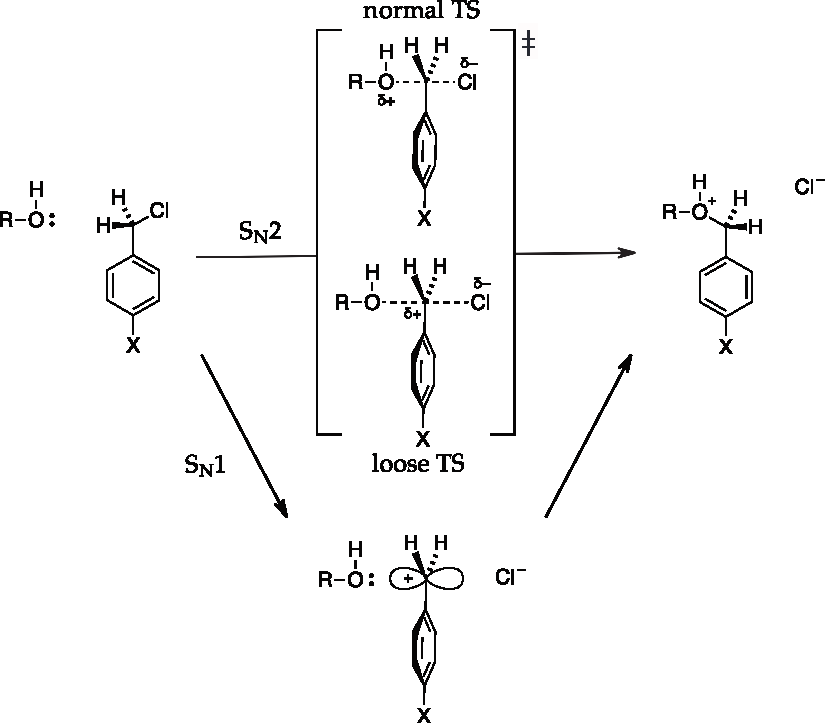
\includegraphics[scale=0.6]{images/BnCl_Mech.pdf}
  \caption[-0mm]{Mechanism scheme for solvolysis of BnCl.  \vspace{2mm} \\  \vspace{20mm} {\sc{\textbf{Personal Exploration Tip:}}} Reinterpretting the authors' schemes can be helpful. Here I try to show how we have two different mechanisms leading to the same product and that the $\rm S_N2$ mechanism can have a changing amount of charge on the benzyl carbon depending on the electron density in the ring. Compare this scheme to scheme~3 in the paper.\tss{1} Can you spot the error in the scheme in the paper?
  
 } 
  \label{fig:mech1}
\end{figure}

In the LFER experiment, we expect a negative reaction constant, $\rho$, of high magnitude for the $\rm S_N1$ mechanism where the rds is formation of the carbocation intermediate. The $\rm S_N2$ mechanism is expected have a negative value with a much smaller magnitude for $\rho$. The authors use the extended Hammett equation and will present two separate values for $\rho$, the reaction constants for inductive effects, $\rho_n$, and for resonance effects, $\rho_r$.  

In a second experiment, the authors examined the selectivity for competing solvent nucleophiles. We expect the cationic $\rm S_N1$ intermediate to become less selective with increasing $\sum \sigma$ (decreasing electron density in the benzene ring). In the $\rm S_N2$ pathway, we expect the reaction to become more selective with increasing $\sum \sigma$ as the activation energy increases due to greater destabilization of the partial positive charge in the reaction centre.

We will see these hypotheses\sidenote[][-50mm]
{These are not really hypotheses anymore. This idea have been supported by experimental evidence since the 1940's. The paper\tss{\ref{ref:1}} is not even an exercise in dotting ``i''s or crossing ``t''s, it is a true reinvention of a wheel. I honestly do not know how this paper was accepted into a journal like ``Physical Organic Chemistry'', which has a strong reputation. Regardless of my haughty opinion, this work does provide an excellent example of how substituent parameters can be used in a mechanistic investigation. Too bad it has all been done before using different methods. \vspace{3mm}}
confirmed as we explore and reproduce the results presented by the authors. Then I will analyze the results using the Yukawa-Tsuno equation and ask the question``why did we bother?''\sidenote[][-8mm]{The authors reference all the relevant previous work in their paper. They aren't ignoring anything. They would likely argue that the value of their contribution is the re-evaluation of this system using the extended Hammett equation. Who am I to judge? Perhaps all truths need to be brought into the light and seen again with the new eyes of the next generation. Let's call this a reboot rather than a sequel.}

\section{The LFER Experiment}

In the paper, the authors present plots of the values for $\log{k_{obs}}$ against $\sum \sigma_m$ for the five series of \textit{para}-substituted benzyl chlorides. The curves drawn on the plots have no meaning and are meant to help the reader visually interpret the plots.  They use the slope of the steepest linear region for each plot (they cherry-picked the two or three points out of five that were linear) to establish a ``limiting'' value for $\rho_n$, the reaction constant for the polar (inductive) effect of substituents in each series. Then they binned the reactants according to \textit{meta} substituents and isolated the term for $\rho_r$ in each case.


\begin{marginfigure}[0mm]
  \centering
    \caption[-0mm]{Figure~2A from the paper\tss{\ref{ref:1}} \label{fig:paperfig2A}}  
    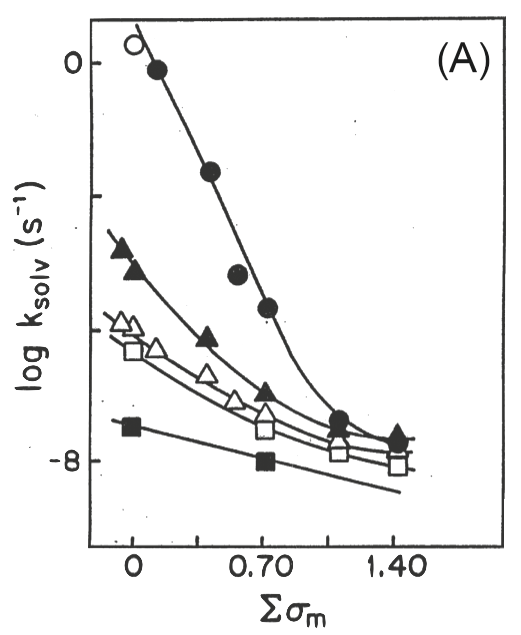
\includegraphics[width=150pt]{images/fig2Apaper.png}
\end{marginfigure}


The conclusion the authors reach is that when the \textit{para} substituent is \ce{p-OMe}, which has a very strong resonance donation to the cationic reaction centre of the intermediate/transition state, we see a $\rho_n$ consistent with the $\rm S_N1$ mechanism. For all other series, the $\rho_n$ has a smaller magnitude consistent with the $\rm S_N2$ mechanism. In the four remaining series, the $\rho_n$ decreases as the $\sigma_r$ value of the \textit{para} substituent decreases, indicating that the structure of the transition state for the $\rm S_N2$ mechanism is becoming ``tighter'' as there is less stabilization of a cationic charge at the benzylic carbon.

\subsection{Reproducing Figure 2A}
I will now use the data and the methods of the authors and will hopefully obtain nearly identical values for $\rho_n$ using the extended Hammett equation. I will plot the values for $\log{k_{obs}}$ against $\sum \sigma_m$ for all five sets on the same plot.\sidenote[][-15mm]{The code for generating the plots is available as a \textit{Python} notebook that accompanies this document. You will be able to see exactly how I calculated values for $\sum \sigma_m$ and how I created the line fits on the plots.}

\begin{figure}[h!]
  \centering
  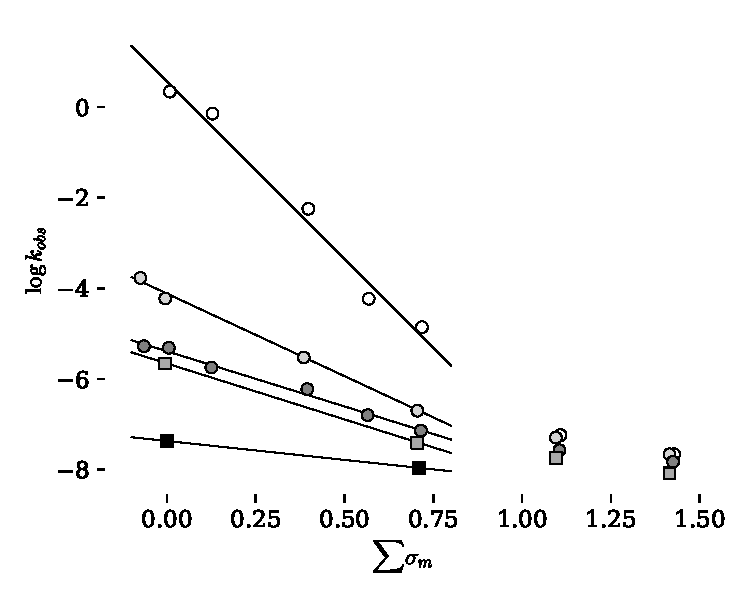
\includegraphics[scale=0.8]{images/plot1.pdf}
  \caption[-0mm]{Reproduction of plot~A in figure~2 of the paper. Hammett plot for the five sets of \textit{para}-substituted benzyl chlorides. Line fits are for data points where $\sum \sigma_m < 0.75$. \vspace{2mm} \\ 
  \ce{p-MeO}: white circles  \\
  \ce{p-Me}: light gray circles  \\
  \ce{p-H}: dark gray circles  \\
  \ce{p-Br}: gray squares   \\
  \ce{p-NO2}: black squares  \\
  
   \vspace{20mm} {\sc{\textbf{Personal Exploration Tip:}}} Reproduce the authors' methods and compare your results to those reported in the paper. Here I am using the ``linear region'' of the plot to establish the value of $\rho_n$ for each series. Am I finding the true linear regions or am I cherry picking data? Judge me harshly.
 } 
  \label{fig:fig2left}
\end{figure}

\clearpage
In figure~\vref{fig:fig2left} is presented a plot of $\log{k_{obs}}$ against $\sum \sigma_m$ for the five sets of reactants grouped by \textit{para}-substituents. The line fits use the ``linear portion'' of the data, which is very much in the eye of the beholder. If my choice of points is the same as the authors I expect to get the same slopes.\sidenote[][-15mm]{Again, if the authors had provided the code that generated their plots then I would know exactly how they picked the linear region.}

\begin{table}[h!]
    \caption[][-0mm]{slopes for the Hammett plots presented in figure~\ref{fig:fig2left}.\\ \vspace{2mm}  \tss{a}The line fits with only two data points have no reportable standard error. \\ \vspace{2mm} \tss{b}When the estimated value at $\sum \sigma_m = 0 $ in this series is omitted, we obtain a value of  $\rho_n = -8.34 \pm 0.79$ \\   \vspace{20mm} {\sc{\textbf{Personal Exploration Tip:}}} A table comparing your own results to the reported values helps the reader to easily compare.}
    
 
 %   \small
    \footnotesize
    \centering
    \fontfamily{ppl}\selectfont
    \sisetup{table-format = 2.2, table-alignment-mode = none, uncertainty-mode = separate}
    \begin{tabular}{@{}l 
                       S[table-number-alignment = center]
                       S[table-number-alignment = left]
                       S[table-number-alignment = left]
                       S[table-number-alignment = left]
                        @{}}
       % \toprule
   & \multicolumn{4}{c}{$\rho_n$ values}  \\
\cmidrule(lr){2-5}
 {Series}   &  {Authors'} & {$\sum \sigma_m < 0.75$} &  {$\sum \sigma_m < 1.25$} & {All data} \\
\midrule
\ce{p-OMe}       & -8.3      &  -7.83 +- 0.58 \tss{b}     &   -7.21 +- 0.43     &  -6.09 +- 0.59    \\
\ce{p-Me}        & -3.6      &  -3.64 +- 0.16      &  -3.06 +- 0.29      &  -2.65 +- 0.29    \\
\ce{p-H}        &  -2.4      &  -2.43 +- 0.12      &   -2.11 +- 0.15    &  -1.83 +- 0.16    \\
\ce{p-Br}         &  -2.0      &  -2.47\tss{a}      &   -1.97 +- 0.42     &   -1.71 +- 0.29    \\
{\ce{p-NO2}}     &  -0.9      &  -0.83\tss{a}      &   -0.83\tss{a}      &  -0.83\tss{a}     \\
        %\bottomrule
    \end{tabular}
    \label{tab:5}
\end{table}

The authors' values agree well with those determined here. The line fits were performed using the linear region of the plots where $\sum \sigma_m < 0.75$. I also performed a line fit with data that included the next point ($\sum \sigma_m < 1.25$) and a line fit that used all the data in each series, despite the obvious curvature in the data. 

The $\rho_n$ value reported by the authors for the \ce{p-OMe} series is significantly greater than my calculated value. I observe in figure~2 of the paper that the point for the highest rate was displayed as an open circle whereas the other points were represented as closed circles. The authors state that this rate was too fast to measure reliably and was estimated. If I omit this data point in the curve fit for $\sum \sigma_m < 0.75$ in the \ce{p-OMe} series, then I observe that $\rho_n = -8.34 \pm 0.79$ 

The value for $\rho_n$ in the \ce{p-Br} series also differs from the reported value. I believe that the authors used an extended linear region for this series (it is a fairly straight line overall) and included the extra point where $\sum \sigma_m < 1.25$.\sidenote[][0mm]{The omitted point in the \ce{p-OMe} series and the extra point in the \ce{p-Br} series were not discussed in the text. I can only guess at what the authors did based on the fact that these changes resulted in $\rho_n$ values that matched the reported values. If the authors had provided their code for the plot as a \textit{Python} notebook, then we would be able to know their exact methodology.}

I cannot explain why my slope for the two-point \ce{p-NO2} series was different than the value reported by the authors (it's two points; where could I have gone wrong?) Perhaps there is a typographical error in the paper?

\subsection{My Own Version of Figure 2A}

Rather than hand-wave some justifications for a set of points in each series that define the ``linear region'', perhaps we could fit the curved lines to a model. The concave-up curves represent two competing processes that are added together to make the value for $k_{obs}$. In the \ce{p-OMe} series, this is the two mechanisms, $\rm S_N1$ and $\rm S_N2$. For the other series, which are all $\rm S_N2$, it is two different geometries of the transition state that we are transitioning between as electron density in the ring changes. The equation used is presented in eq.~\ref{eq:1}

\begin{equation}
\begin{split}
\log{k_1} &= \rho_1 \sum \sigma_n + c_1 \\
\log{k_2} &= \rho_2 \sum \sigma_n + c_2 \\
\log{k_{obs}} &= \log\left(k_1 + k_2\right)
\label{eq:1}
\end{split}
\end{equation}

I will use a curve fit tool,\sidenote[][0mm]{And, of course, this curve fit is documented by providing the code in the supplementary \textit{Python} notebook and accompanies this document. I don't have to explain the curve fit because the code explains it for me.} We will get the values for $\rho_1$, $c_1$, $\rho_2$, and $c_2$ that result in the best fit to the data. This will be the slope and intercept of the two Hammett relationships that we are summing together to explain the curve of the line. For the \ce{p-NO2} series, which has only two points, I used a linear fit. For the \ce{p-Br} series, which has four points for a four-parameter curve fit, I had to set $c_1$ to the value observed at $\sum \sigma_n = 0$ (the line will now be forced to pass through this point). I had to do that because the curve-fit algorithm required more data points than parameters. The value of $\rho_1$ was constrained and it reached the limit of the constraint ($-2.5$). With only a single point defining $\rho_1$ in this series the slope from the curve fit is essentially a random number unless it is constrained to a reasonable range.\sidenote[][-20mm]{I don't have to write another paragraph explaining exactly how the line fits were adjusted because the reader can refer to the \textit{Python notebook} that documents my data analysis. Providing such documentation actually saves me time in explaining my methods.}

\begin{figure}[h!]
  \centering
  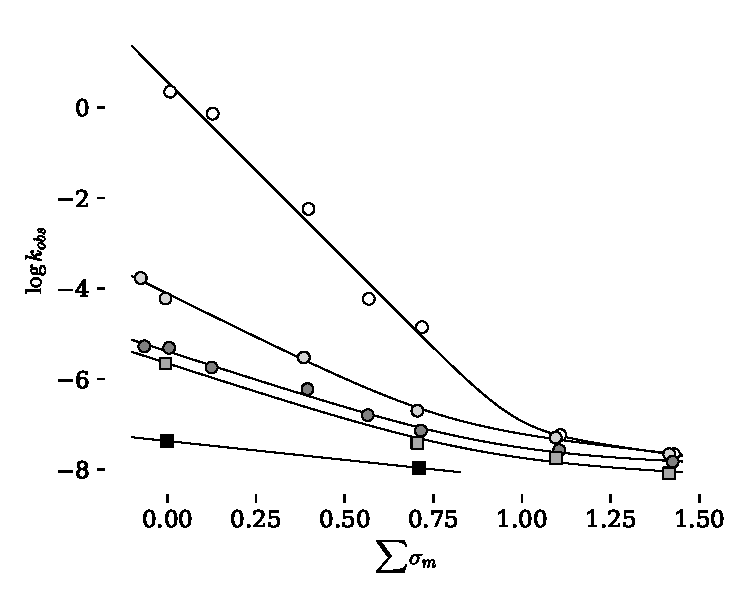
\includegraphics[scale=0.8]{images/plot2.pdf}
  \caption[-0mm]{Reproduction of plot~A in figure~2 of the paper. Hammett plot for the five sets of \textit{para}-substituted benzyl chlorides. Line fits are for plotted according to the best fit parameters for the model described by eq.~\ref{eq:1}. \vspace{2mm} \\
  \ce{p-MeO}: white circles  \\
  \ce{p-Me}: light gray circles  \\
  \ce{p-H}: dark gray circles  \\
  \ce{p-Br}: gray squares   \\
  \ce{p-NO2}: black squares  \\
  
 } 
  \label{fig:fig2left_MyOwn}
\end{figure}



\begin{table}[h!]
    \caption[][-0mm]{Curve fit values for the Hammett plot model presented eq.~\ref{eq:1} and plotted in figure~\ref{fig:fig2left_MyOwn}.\\ \vspace{2mm}  \tss{a} Curve fit modified with parameter constraints. See \textit{Python} notebook for details. \\ \vspace{2mm} \tss{b}The line fits with only two data points have no reportable standard error.}
    
 
 %   \small
    \footnotesize
    \centering
    \fontfamily{ppl}\selectfont
    \sisetup{table-format = 2.2, table-alignment-mode = none, uncertainty-mode = separate}
    \begin{tabular}{@{}l 
                       S[table-number-alignment = center]
                       S[table-number-alignment = left]
                       S[table-number-alignment = left]
                        @{}}
       % \toprule
   &  &  \multicolumn{2}{c}{Curve fit values}  \\
\cmidrule(lr){3-4}
 {Series}   &  {Authors'} & {$\rho_1$} &  {$\rho_2$}  \\
\midrule
\ce{p-OMe}       & -8.3      &  -7.84 +- 0.58     &   -1.11 +- 1.67   \\
\ce{p-Me}        & -3.6      &  -3.87 +- 0.33      &  -0.84 +- 0.53           \\
\ce{p-H}        &  -2.4      &  -2.54 +- 0.12      &   -0.27 +- 0.67          \\
\ce{p-Br}         &  -2.0      &  -2.5 +- 0.67\tss{a}      &   -0.30 +- 1.3       \\
{\ce{p-NO2}}     &  -0.9      &  -0.83\tss{b}      &   {--}           \\
        %\bottomrule
    \end{tabular}
    \label{tab:6}
\end{table}

We see that the value of $\rho_n$ for the more activated cases ($\sum \sigma_m \le 0.5$) is described by the value of $\rho_1$ in table~\vref{tab:6}. The uncertainty is very large, as expected with a multi-parameter plot where the data does not exceed the number of parameters by much. The values of $\rho_1$ track very well with the authors' $\rho_n$ values obtained from linear plots in the ``linear regions.'' The value of $\rho_2$, which describes the value of $\rho_n$ in deactivated systems ($\sum \sigma_m \ge 1.0$), approaches a small magnitude, indicating much less positive charge at the reaction centre in the transition state. The values of $\rho_1$ have extremely large uncertainties and I can understand why the authors chose to ignore it. More data points would help. 



\subsection{Reproducing Figure 2B}

\begin{marginfigure}[0mm]
  \centering
    \caption[-0mm]{Figure~2B from the paper\tss{\ref{ref:1}} \label{fig:paperfig2B}}  
    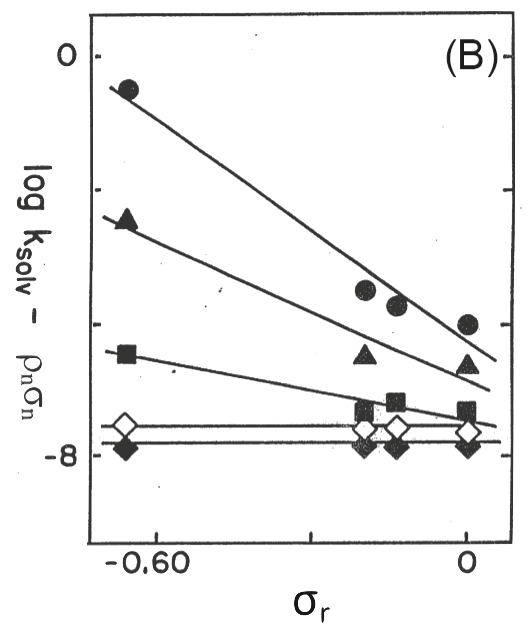
\includegraphics[width=150pt]{images/fig2Bpaper.png}
\end{marginfigure}


The extended Hammett equation can be rearranged so that we can plot $\log{k_{obs}}-\rho_n \sigma_n$ vs $\sigma_r$ and the slope of the line will give us $\rho_r$.  We established the sensitivity to the polar effect of substituents by using only \textit{meta} substituents where we knew that $\rho_r = 0$. We now have a value for $\rho_n$ in each series of \textit{para}-substituted benzyl chlorides in figure~\vref{fig:fig2left} and figure~\vref{fig:fig2left_MyOwn} and reported in table~\vref{tab:5} and table~\vref{tab:6}. Now that we have values for $\rho_n$ for each series, we can now isolate the polar effect of the \textit{para} substituent from the resonance effect. We have values for $\rho_n$ and $\sigma_n$ and $\sigma_r$ values are listed in table~\vref{tab:3}. 

\begin{figure}[h!]
  \centering
  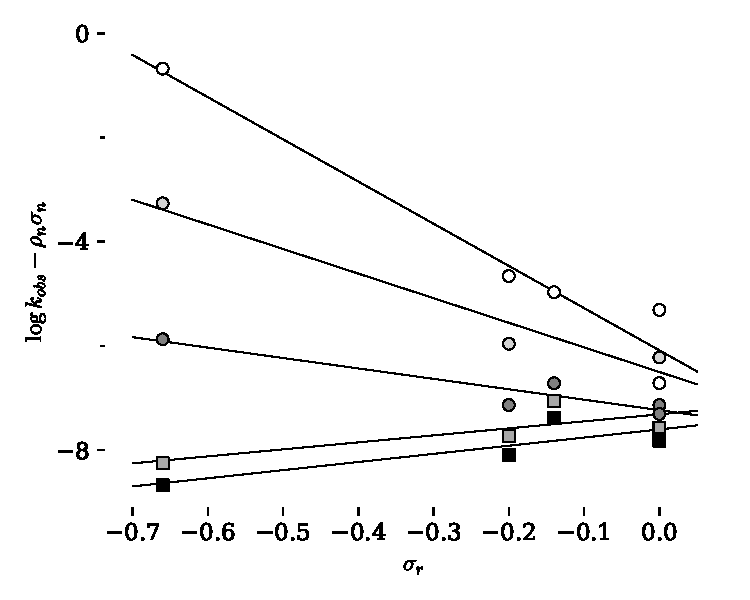
\includegraphics[scale=0.8]{images/plot4.pdf}
  \caption[-0mm]{Reproduction of plot~B in figure~2 of the paper. Hammett plot for five sets of \textit{meta}-substituted benzyl chlorides as the \textit{para} substituent is varied.  \vspace{2mm} \\
  {m-H,H}: white circles  \\
  {m-H,Br}: light gray circles  \\
  {m-H,\ce{NO2}}: dark gray circles  \\
  {m-Br,\ce{NO2}}: gray squares   \\
  {m-\ce{NO2},\ce{NO2}}: black squares  \\
  
   \vspace{20mm} {\sc{\textbf{Personal Exploration Tip:}}} Sometimes your analysis and the results of the authors will differ. Somebody made a mistake here, most likely me. However, I can't see why the {m-Br,\ce{NO2}} and {m-\ce{NO2},\ce{NO2}} sets differ so much from the authors values when the other three are fairly close. Document your own calculations so that the reader can check your work, at least. 
 } 
  \label{fig:fig2B_MyOwn}
\end{figure}

\begin{table}[h!]
    \caption[][-0mm]{Curve fit values for the Hammett plot model presented eq.~\ref{eq:1} and plotted in figure~\ref{fig:fig2left_MyOwn}.\\ \vspace{2mm}  \tss{a} reported in the paper as $\sigma_{m_{Br}} = 0.28$. This was not a typo as it also results in the incorrect value of $\sum \sigma_m = 0.99$ for the {m-Br,\ce{NO2}} series. \\ \vspace{2mm} \tss{b}In the {m-H,H} series, the authors do not include the data point for p-\ce{NO2}-benzyl chloride. If you go to the $Python$ notebook and remove the p-\ce{NO2} series from the data then you will get a slope of $-7.5$. If you further replace my value for $\rho_n$ with the authors' value of $-8.3$, then the slope is $-7.3$. By providing the notebook, I enable the reader to go there and fool around with the data. Break things and learn -- it is the way.}
    
 
 %   \small
    \footnotesize
    \centering
    \fontfamily{ppl}\selectfont
    \sisetup{table-format = 10.10, table-alignment-mode = marker, uncertainty-mode = separate}
    \begin{tabular}{@{}l 
                       S[table-number-alignment = center]
                       S[table-number-alignment = left]
                       S[table-number-alignment = center]
                        @{}}
       % \toprule
   &  &  \multicolumn{2}{c}{$\rho_r$ values}  \\
\cmidrule(lr){3-4}
 {Series}            & {$\sum sigma_m$}  &  {Authors'}       & {from figure \ref{fig:fig2B_MyOwn}}   \\
\midrule
{m-H,H}               &  0               & -7.2               &  -8.10 +- 1.08\tss{b}          \\
{m-H,Br}              &  0.39\tss{a}     & -4.7               &  -4.72 +- 1.06                 \\
{m-H,\ce{NO2}}        &  0.71            &  -1.9              &  -2.00 +- 0.43                 \\
{m-Br,\ce{NO2}}       &  1.10\tss{a}     &  -0.2              &  1.35 +- 0.77                  \\
{m-\ce{NO2},\ce{NO2}} &  1.42            &  {$\approx 0$}      &  1.46 +- 0.74                 \\
        %\bottomrule
    \end{tabular}
    \label{tab:7}
\end{table}

Plotting the value of $\log{k_{obs}}$ and subtracting the value created by multiplying the $\sigma_n$ value of the \textit{para} substituent with the  $\rho_n$ value for the series that featured that \textit{para} substituent  will give us a (hopefully) straight line with a slope of $\rho_r$. We can repeat this plot with any series of benzyl chlorides where only the \textit{para} substituent is changing.  The authors identified such series within their data set and plotted them as shown in figure~2B of the paper.\tss{\ref{ref:1}} Each series features the same set of \textit{meta} substituents.

I plotted the same data and used the values from table~\ref{tab:5} for the linear regions of the plots. I plotted this data in figure~\vref{fig:fig2B_MyOwn}. The slopes, which equate to the $\rho_r$ values for each series are listed in table~\vref{tab:7}, are nearly identical to the authors' values except for the two least activated series (where the \textit{meta} substituents are most electron-withdrawing). In these two cases my results differ markedly from the authors' and I cannot explain it. I have no access to the parameters or the calculations used by the authors to calculate the value of $\log{k_{obs}}-\rho_n \sigma_n$ but I did get the textbook that they referenced\tss{\ref{ref:8}} and I believe that I used the correct parameters from tables in that book. However, since the data analysis was not documented, I can't say why the author's results differ from my own for only those two series.\sidenote[][-20mm]
{The authors do state the ``The data that support the findings of this study are available from the corresponding author upon reasonable request.'' Would they consider an email requesting all their data and all their calculations to be reasonable? If the plots and calculated results were created in \textit{Python} notebooks and posted on the journal website as supplementary material, then I would have been easily able to see how they are right and I am wrong. Instead I am left to entertain conspiracy theories that positive slopes worked against their hypothesis and were somehow avoided.\vspace{2mm}}

\section{The Product Analysis Experiment}

The authors performed a competition experiment where they carried out the solvolysis in a solvent mixture that contain three nucleophiles: methanol, trifluoroethanol and water mixed in a 3/27/70 ratio. They calculated the relative rate constants from the observed product ratios and the know concentrations of the nucleophiles.\sidenote[][-0mm]
{No, there is no information on how this was done, but it seems reasonable. It would be nice to have the raw product-ratio data so that we could check the math. I hope you will provide all your data in supplementary material when you publish.}  The results are presented in table~\ref{tab:1} \vpageref{tab:1}.

The hypothesis is that the more nucleophilic solvents will show a higher rate constant for addition to the benzyl chloride or a cationic intermediate. A cationic intermediate in an $\rm S_N1$ mechanism would show less selectivity as the ring becomes more electron-deficient in each series of \textit{para} substituted benzyl chlorides. For the $\rm S_N2$ mechanism, the selectivity should increase with decreasing electron density as this results in a ``tighter'' transition state that benefits from a stronger nucleophile. 

The authors present their plots for each series in figures~3 and 4 of the paper\tss{\ref{ref:1}} and I will not reproduce them here. The \ce{p-OMe} series shows a negative slope in selectivity ($\log{\nicefrac{(k_{MeOH}}{k_{TFE}}}$ vs $\sum \sigma_m$) for the five data points where $\sum \sigma_m \le 0.75$. This is indicative of a true carbocation intermediate and an $\rm S_N1$ mechanism. The two data points in the range of $\sum \sigma_m > 0.75$ slope upwards showing the expected increase in selectivity as expected of a transition state defining a $\rm S_N2$ mechanism. All the other series showed positive slopes indicating the expected $\rm S_N2$ TS and showed slight to pronounced curvatures, indicating progressive changes in the TS structure.

\subsection{Reproducing Figures 3 \& 4}

I will plot the data for figures~3 and 4 in the paper all in a single plot as shown in figure~\vref{fig:fig3-4_paper}. 

\begin{figure*}[h!]
  \centering
  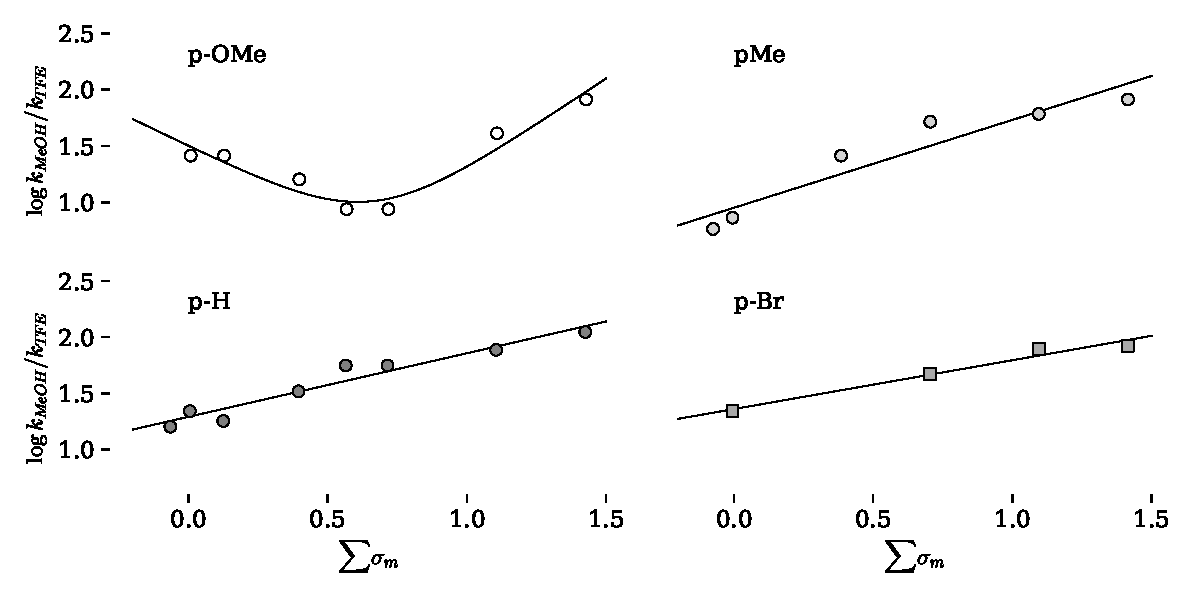
\includegraphics[scale=0.8]{images/plot6.pdf}
  \caption[-0mm]{Reproduction of the plots in figures~3 \& 4 of the paper.   \vspace{2mm} \\
 } 
  \label{fig:fig3-4_paper}
\end{figure*}

The \ce{p-OMe} series show the switch from a $\rm S_N1$ to a $\rm S_N2$ mechanism. All the other plots indicate a $\rm S_N2$ mechanism. The authors draw curved lines for all the plots but a straught line looks perfectly good for the \ce{p-H} and the \ce{p-Br} series. None of the lines on the plots are meant to provide any meaningful parameters, they are just there to guide you eye.\sidenote[][0mm]{The \ce{p-NO2} series is not included in figure~\vref{fig:fig3-4_paper}}

\section{Using the Hammett Equation}

The authors establish the $\rho_n$ using a slope from the plot of $\log{k_{obs}}$ against $\sum \sigma_m$. Then the establish a value for $\rho_n$ in the case of each \textit{para}-substituted series. Can we find a simper method where we use the data as a whole rather than separating it into five series?

\subsection{A Holistic Hammett Plot}

Let us plot $\log{k_{obs}}$ vs the total Hammett substituent parameters for the ring, both \textit{para} and  \textit{meta}, $\sum \sigma_{p,m}$. This plot is presented in figure~\vref{fig:YK2}.

We can see that the data in each series overlaps into a nice trend except for the five points in the \ce{p-OMe} series that we associated with the change to a $\rm S_N1$ mechanism. I believe that we can clearly see now that there is one mechanism for the majority of the reactants and that the most activated of the \ce{p-OMe} series has a different mechanism.

I binned the data into two groups, the $\rm S_N1$ and the $\rm S_N2$ group. I fit the five points of the \ce{p-OMe} series that are hypothesized to represent the $\rm S_N1$ mechanism to a linear model and determine the slope. I fit the remaining data, which is hypothesized to be $\rm S_N2$, to a four-parameter curve fit that expresses the model from eq.~\vref{eq:1} for moving from one mechanism (or TS structure) to another. The slopes are each end represent the reaction constants for the extreme forms of the TS in this continuum. 

\begin{figure}[h!]
  \centering
  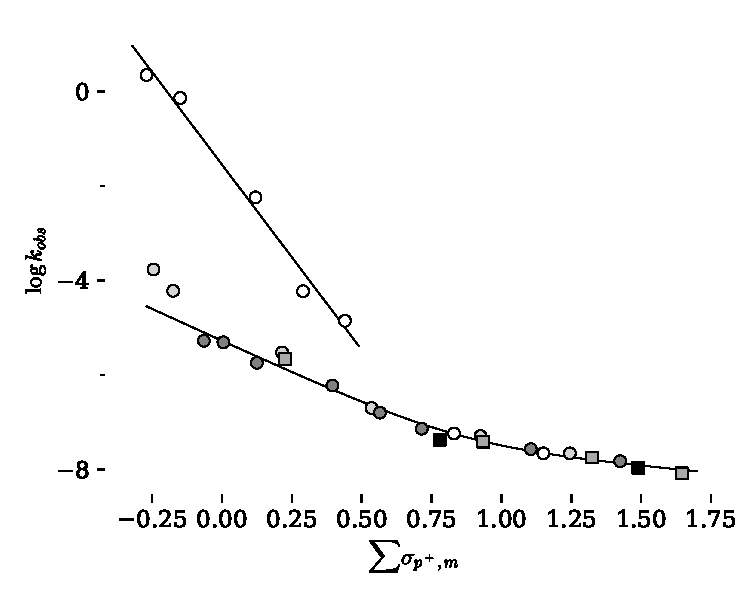
\includegraphics[scale=0.8]{images/plot9s.pdf}
  \caption[-0mm]{Hammett plot for the entire dataset of benzyl chlorides.  \vspace{2mm} \\ 
  \ce{p-MeO}: white circles  \\
  \ce{p-Me}: light gray circles  \\
  \ce{p-H}: dark gray circles  \\
  \ce{p-Br}: gray squares   \\
  \ce{p-NO2}: black squares   \vspace{2mm}  \\

    {$\rm S_N1$}  \\
    \hspace{3mm} $\rho = -7.83 \pm 0.58$ \vspace{2mm} \\
    {$\rm S_N2$}  \\
    \hspace{3mm} $\rho = -2.71 \pm 0.30$  \\
    \hspace{3mm} $\rho = -0.55 \pm 0.37$ \vspace{2mm} \\

     \vspace{20mm} {\sc{\textbf{Personal Exploration Tip:}}} If you think there is a clearer way to present data then give it a try. Here I plotted the $\log{k_{obs}}$ against $\sum \sigma$ value for each ring. Does this highlight the differences of the {p-\ce{MeO}} series better than keeping all the plots separate? Does it reveal some extra details such as how the rightmost two points of the {p-\ce{MeO}} series are likely $\rm S_N2$ and the leftmost two points in the {p-\ce{Me}} series may be $\rm S_N1$? Sometimes a new point of view can reveal unseen information -- or fool us with illusions.
 } 
  \label{fig:YK2}
\end{figure}

The large negative slope of $-7.8$ for the $\rm S_N1$ mechanism is expected for an unsubstituted benzylic carbon. The carbocation intermediate is high in energy and electronic effects will be large. This also agrees with the $\rho_n$ values as this is essentially the same data series as in the previous analysis above. It is a series of \textit{para} substituted benzyl chlorides with differing \textit{meta} substitutions. The data set is that of the linear region in the extended Hammett analysis we were exploring above. The Hammett plot for the $\rm S_N2$ mechanism also gives similar results to the previous work. The largest slope is at the most activated end of the plot (more negative values for $\sum \sigma$) and the smallest slope is at the least activated end (more negative values for $\sum \sigma$). The values of $-2.7$ and $-0.6$ are in agreement with the observations above. Observe that the left-most points in the \ce{p-Me} series are above the line. Perhaps these are $\rm S_N1$ as well?

\subsection{A Brown-Okamoto Plot}

The rates for the putative $SN_1$ mechanism in the \ce{p-OMe} series were well above the line of the rates in the data representing the $SN_2$ mechanism. If the outliers were experiencing a greater sensitivity to resonance donation by the \ce{p-OMe} substituent then perhaps we should use the Brown-Okamoto $\sigma^+$ substituent parameter in place of the Hammett $\sigma_p$ parameter. 

I will construct a new plot where the sum of sigma values is created using the $\sigma^+$ and $\sigma_{m}$ from table~\vref{tab:2}.\sidenote[][-25mm]{Full disclosure: I used the values in the database that I have on the GitHub site. They happen to be the same as the values from the textbook reference\tss{\ref{ref:8}} used in table~\ref{tab:2}. I don't really have to add this note because all the calculations and data for the plots are documented in the \textit{Python} notebooks that accompany this report. You can easily see how my words match my deeds (or not) by examining the code.} You can see in figure~\vref{fig:YK3} that the data seems to coalesce into a single trend. Should I be fitting this to two separate models as shown? Or should I try to establish a more complete model?

\begin{figure}[h!]
  \centering
  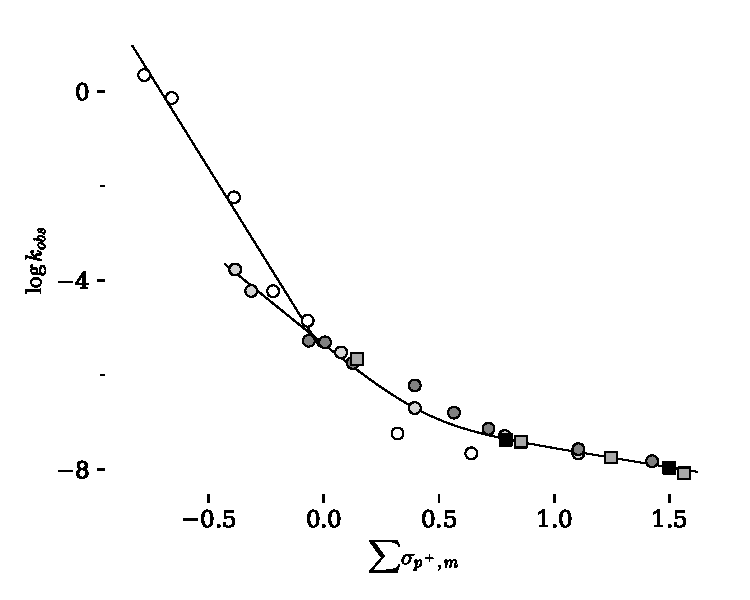
\includegraphics[scale=0.8]{images/plot9.pdf}
  \caption[-0mm]{Brown-Okamoto plot for the entire dataset of benzyl chlorides.  \vspace{2mm} \\
    \ce{p-MeO}: white circles  \\
  \ce{p-Me}: light gray circles  \\
  \ce{p-H}: dark gray circles  \\
  \ce{p-Br}: gray squares   \\
  \ce{p-NO2}: black squares  \vspace{2mm}  \\

    {$\rm S_N1$}  \\
    \hspace{3mm} $\rho = -7.83 \pm 0.58$ \vspace{2mm} \\
    {$\rm S_N2$}  \\
    \hspace{3mm} $\rho = -3.98 \pm 0.46$  \\
    \hspace{3mm} $\rho = -0.80 \pm 0.27$ \vspace{2mm} \\

   
 } 
  \label{fig:YK3}
\end{figure}

Also, I note that the $\sigma^+$ do not seem to go far enough to bring the \ce{p-OMe} series all the way over to connect with the $\rm S_N2$ series. the slope for the $\rm S_N1$ \ce{p-OMe} series did not change as every case was identical at the \textit{para} position and all shifted by the same amount.

In figure~\vref{fig:YK3} we can see that the least activated pair of points in the \ce{p-OMe} series is being pulled out of the trend when we switched from $\sigma$ to $\sigma^+$ as the basis for the substituent parameters. These two points are for reactants that are proposed to undergo the $\rm S_N2$ mechanism and do not have the same resonance connection as the $\rm S_N1$ part of the series. 

I also note that the two most activated points in the \ce{p-OMe} series are to the left of $\sum \sigma$ values that include the $\rm S_N1$ mechanism. We did not detect an $S_N1$ effect in the product analysis in a solvent system of \qty{70}{\percent} water/methanol (with a little bit of TFE). The rate data was performed in \qty{80}{\percent} water/acetonitrile. The two solvent systems have very similar abilities to stabilize carbocations according to their Grunwald-Winstein $Y_{OTs}$ solvent parameters.\sidenote[][0mm]{See chapter~8.4 of the class textbook. \vspace{2mm}} For the methanol mixture $Y_{OTs} = 2.97$ and for the acetonitrile mixture $Y_{OTs} = 2.7.$\sidenote[][0mm]{``Y\textsubscript{X} Scales of Solvent Ionizing Power.'' T.W. Bentley and G. Llewellyn, \textit{Progress in Physical Organic Chemistry}, \textbf{1990},  \textit{17}, 121-158. \url{https://doi.org/10.1002/9780470171967.ch5} \label{ref:26}} The two solvent systems will have similar likelyhood of the $\rm S_N1$ mechanism.

\section{A Yukawa-Tsuno Approach}

\marginnote[5mm]{The Yukawa-Tsuno equation 
\begin{equation*}
\log{\frac{k_X}{k_H}} = \rho \left[ \sigma + r \left(\sigma^+ - \sigma \right) \right]
\end{equation*}
}


I propose a hypothesis that the two least activated examples in the \ce{p-Me} series are undergoing $\rm S_N1$ hydrolysis and that they should be grouped with the $\rm S_N1$ set of the \ce{p-OMe} series. The $\rm S_N1$ set of data will have a different dependance on resonance contributions from \textit{para} substituents than the $\rm S_N2$ set. 

The Yukawa-Tsuno equation\sidenote[][0mm]{See chapter~8.3 of the class textbook. \vspace{2mm}} may be appropriate here. There seems to be an even greater dependance of resonance that can be explained by the $\sigma^+$ parameters. The literature reports that the Yukawa-Tsuno $r$-value for benzhydryl chloride (\ce{Ph2CHCl} hydrolysis is 1.23 in \qty{100}{\percent}~methanol.\sidenote[][0mm]{``Resonance Effect in Hammett Relationship. III. The Modified Hammett Relationship for Electrophilic Reactions.'' Yasuhide Yukawa, Yuho Tsuno, \textit{Bull. Chem. Soc. Japan}, \textbf{1959}, \textit{32}, 971–981. \url{https://doi.org/10.1246/bcsj.32.971} \vspace{2mm}} This is explained as the benzhydryl carbocation in methanol being less stable than the cumyl cation in water upon which the $\sigma^+$ scale is based.  

Looking back to the plots for the hydrolysis of benzyl chloride in \qty{50}{\percent} water/alcohol mixtures that have been presented in class\sidenote[][0mm]{See the ``Linear Free Energy Relationships. Part 1.'' handout and tables~4 and 5 within. \vspace{2mm}} we do see that the most activated point (\ce{p-OMe}) is above the line and that there is a subtle curve that does not quite rise to the need to abandon a linear analysis. This study is performed in more polar conditions\sidenote[][0mm]{In \qty{50}{\percent} ethanol, $Y_{OTs} = 1.29$ compared to \qty{20}{\percent}acetonitrile used by the authors where $Y_{OTs} = 2.7.$\tss{\ref{ref:26}}} where cationic character on the benzylic carbon in the $\rm S_N2$ TS (and the switch to a carbocation intermediate in an $\rm S_N1$ mechanism) is more likely.

\subsection{The Plan for Data Analysis}

I am going to include the two most activated members of the \ce{p-Me} series with the already selected $\rm S_N1$ points of the \ce{p-Me} series. Then I will perform a curve fit optimization that will find the optimal $r$ value to fit all the points on a straight line. I will take all the other points as a set representing the $\rm S_N2$ mechanism and fit them to the model described by eq.~\ref{eq:1} while optimizing for the $r$ value.  I will now have values for the Yukawa-Tsuno $r$ factor for both cases. 

Once I have these $r$ values, I will calculate the values of $\sigma_{calc} = \sum \sigma + r(\sigma^+ - \sigma)$ for each reactant. I will now have a data set of the $\log{k_{obs}}$ values and the calculated values for $\sigma_{calc}$ using the $r$ value according to the assigned mechanism. I will then make a final plot of $\log{k_{obs}}$ vs $\sigma_{calc}$. I will then attempt to fit this new unified set of data against a model that adds the rates of $\rm S_N1$ and $\rm S_N2$ pathways together. 

\subsection{Optimizing for $r$ values in the $\rm S_N1$ regime}

In past examples where we have optimized for the Yukawa-Tsuno $r$-value I maximized the correlation constant of the line fit, $R^2$.\sidenote[][0mm]{See the ``LFER Part 2: Substituents with More Punch'' handout and plots within. \vspace{2mm}} Lets us try that again. The difference between

In figure~\vref{fig:YK4} is plotted the set of data that is believed to feature the $\rm S_N1$ mechanism (as discussed above). The plot show line fits for the Yukawa-Tsuno equation with values of $r$ set at $0$, $1.0$ and $1.4$. Observe that the effect of increasing the $r$ value is to create a new composite $\sigma$ value between (and, in this case, beyond) $\sigma$ and $\sigma^+$ (or $\sigma^-$). The \ce{p-OMe} series has a much greater difference between $\sigma$ and $\sigma^+$ than the \ce{p-Me} series. the effect of increasing $r$ is to move the calculated $\sum \sigma$ value to the left with the \ce{p-OMe} series moving to a greater extent. the optimal $r$ value will be when the two set of data ``line up.''

The optimization plot of $R^2$ score vs $r$ value is presented in figure~\vref{fig:YK4R}. We see that there is a significant difference in the score for the line fit and that the optimal $r$ value is certainly above $1.0$.

The difference between $\sigma$ and $\sigma^+$ is large for \ce{p-OMe} and \ce{p-Me} and so it is easy to obtain an $r$ value in systems that involve resonance donation to the reaction centre. Carbocations are the definition of such a case. The value of $r = 1.40$ established by optimizing the $R^2$ score of the line-fit w.r.t. $r$ is reasonable. The Brown-Okamoto $\sigma^+$ values were established using a completely substituted carbocation and the unsubstituted benzyl carbocation will require more resonance stabilization than the dimethylbenzyl (cumyl) cation.

We now have a data set for the $\rm S_N1$ data points. For these data points, the $x$ and $y$ values will be $\sigma + 1.4 \left(\sigma^+ - \sigma \right)$ and $\log{k_{obs}}$. Now let us consider the $\rm S_N2$ data.

\begin{figure}[h!]
  \centering
  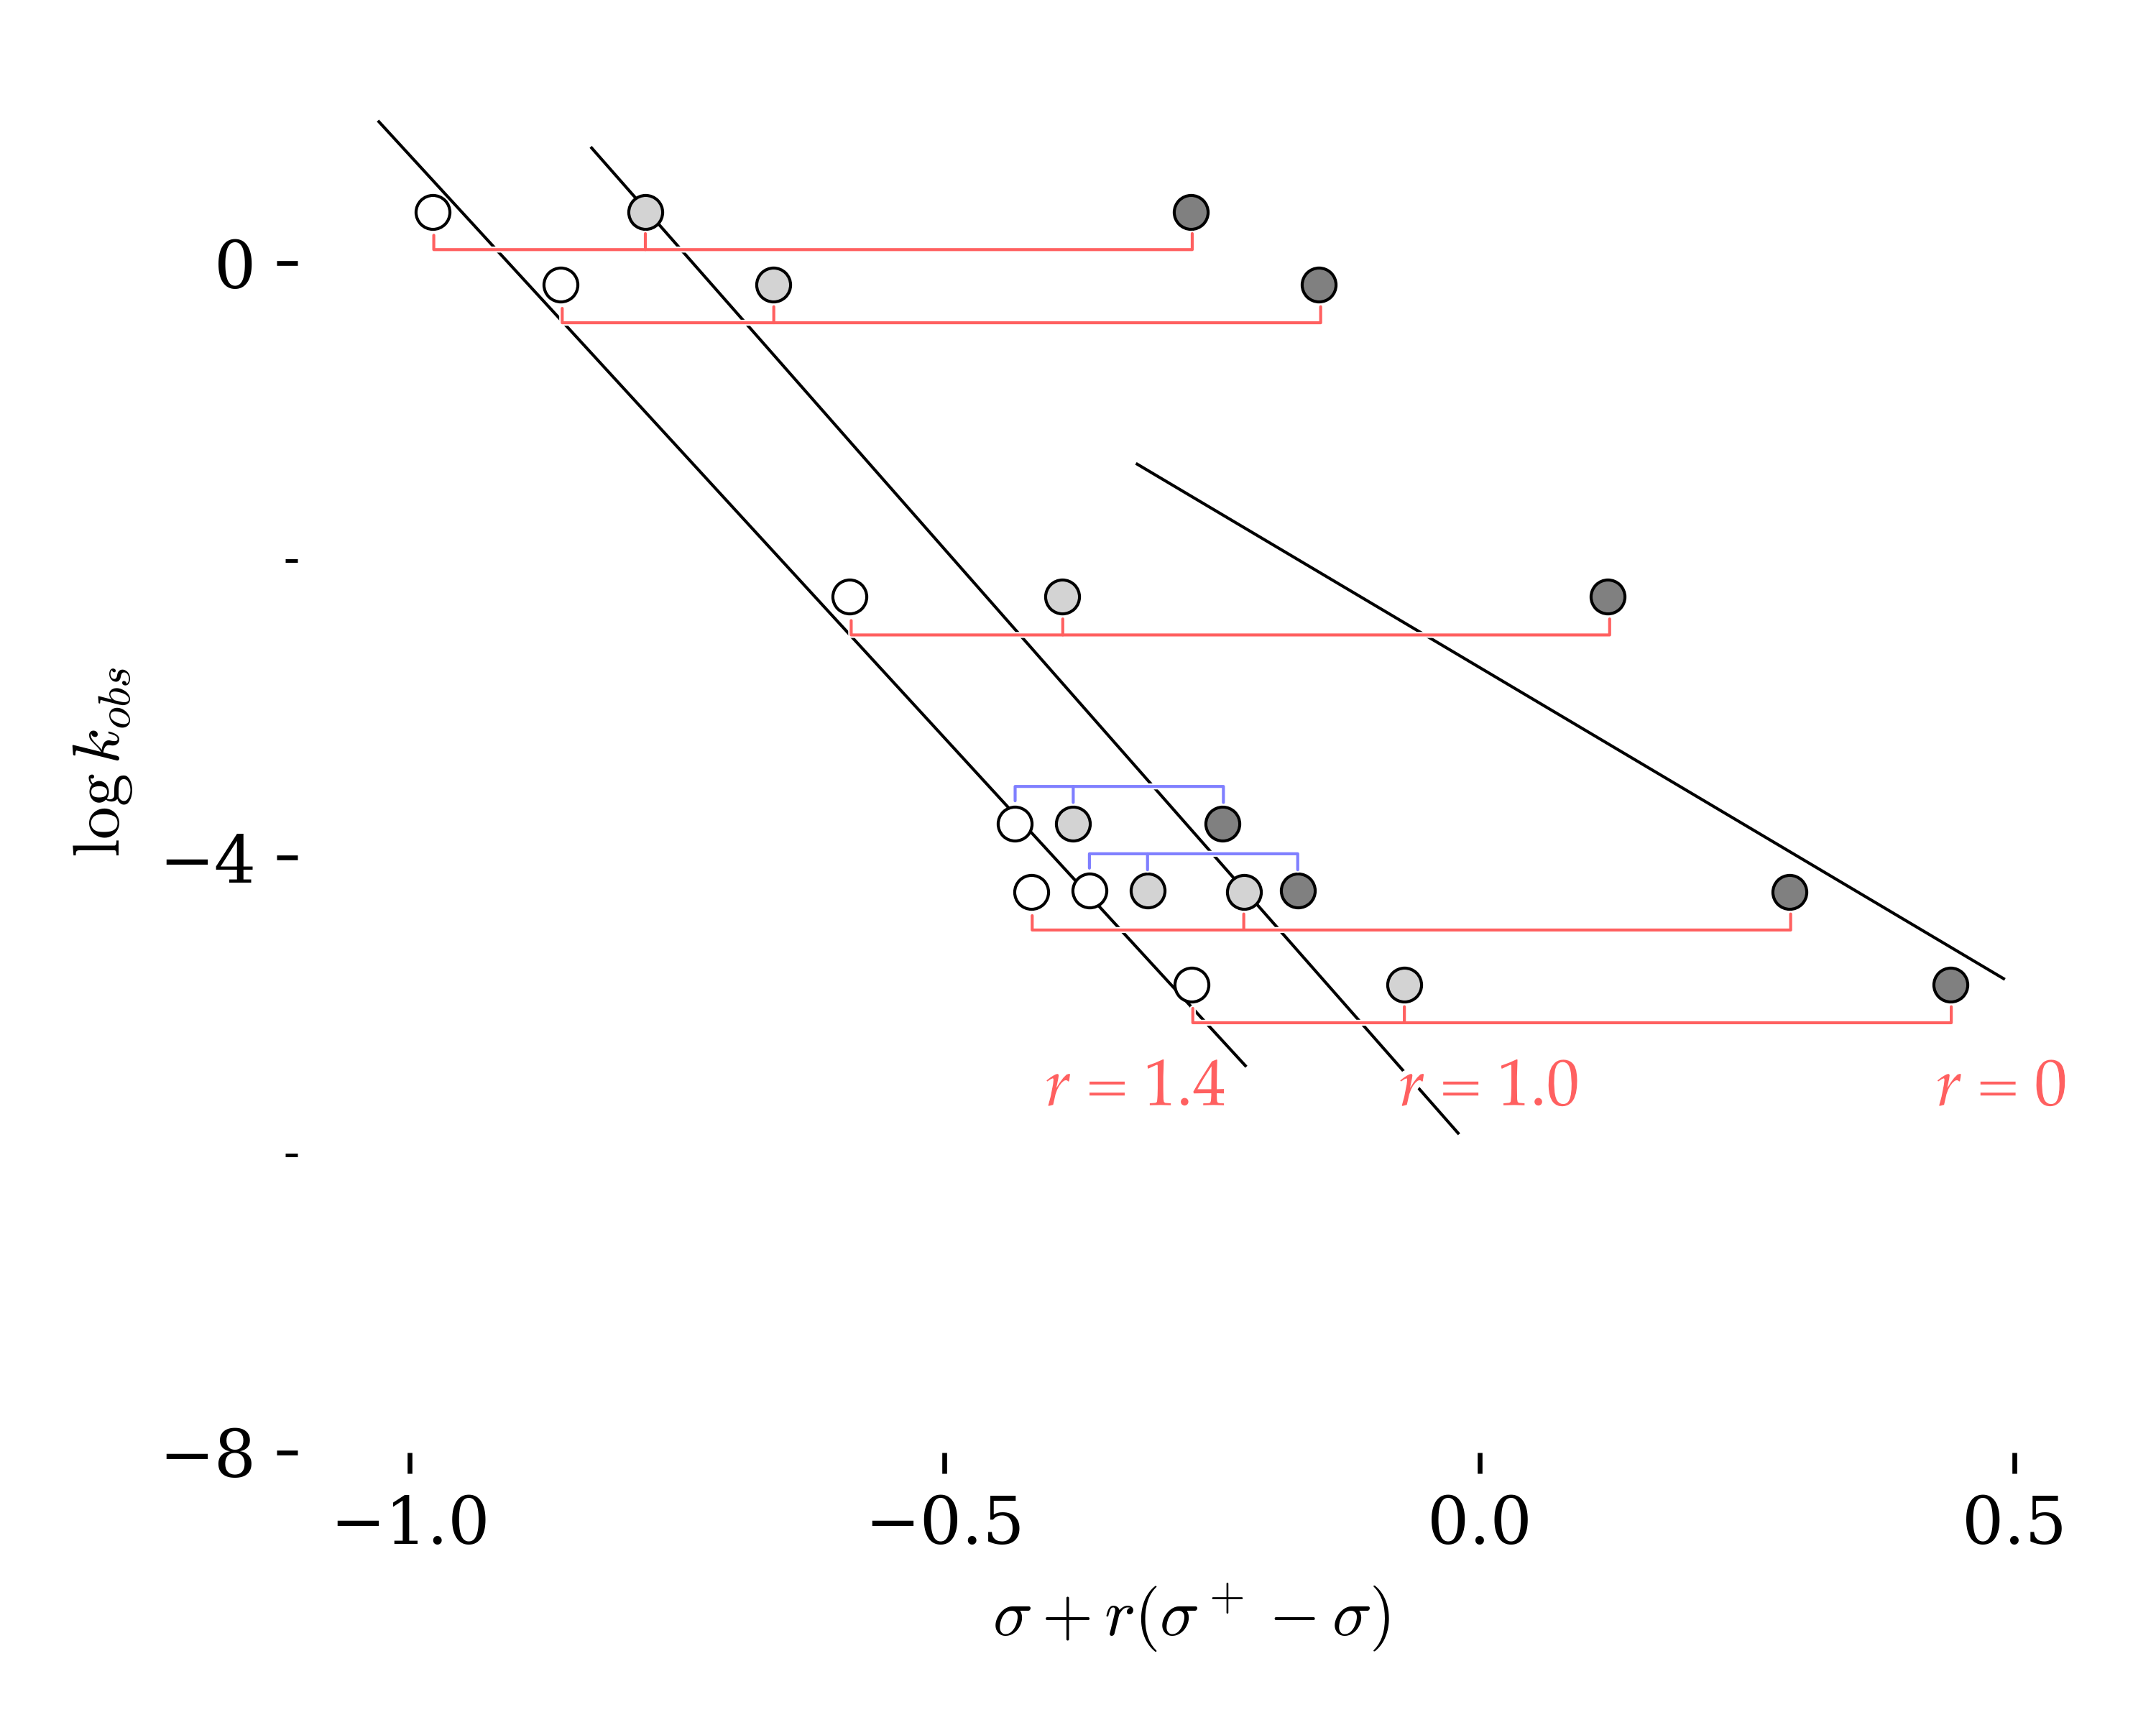
\includegraphics[scale=0.8]{images/plot10_multiR.png}
  \caption[-5mm]{Yukawa-Tsuno plot for the $\rm S_N1$ set of rates.   \vspace{2mm} \\
  {$r = 1.4$}: white circles  \\
  \hspace{3mm} $\rho = -7.84 \pm 0.41$, $R^2 = 0.987$ \vspace{2mm} \\
  {$r = 1.0$}: light gray circles  \\
  \hspace{3mm} $\rho = -8.18 \pm 1.11$, $R^2 = 0.917$ \vspace{2mm} \\
  {$r = 0.0$}: dark gray circles  \\
  \hspace{3mm} $\rho = -4.27 \pm 2.73$, $R^2 = 0.327$ \vspace{2mm} \\

   
 } 
  \label{fig:YK4}
\end{figure}

\begin{marginfigure}[-25mm]
  \centering
    \caption[-0mm]{Optimizing $r$ for the Yukawa-Tsuno plot \label{fig:YK4R}}  
    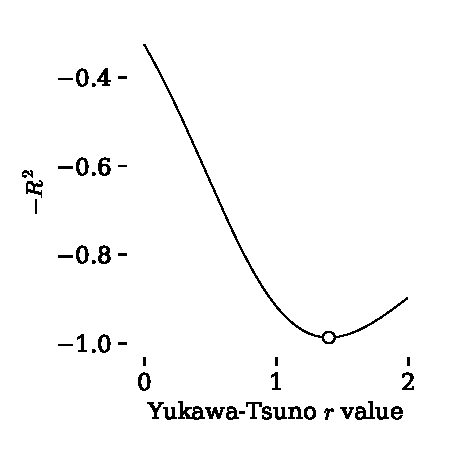
\includegraphics[width=150pt]{images/plot10R.pdf}
\end{marginfigure}



\subsection{Optimizing for $r$ values in the $\rm S_N2$ regime}

Let us now take the data for the $\rm S_N2$ region of the Hammett plot. We will use a $\sigma$ value as determined using the Yukawa-Tsuno equation. Figure~\vref{fig:YK5} show the data plotted using $r = 0.21$, which was the optimal value. The same data plotted using $r = 0$ is presented with black circles. You can see that there is little difference as most of the \textit{para} substituents in this set have little or no difference between $\sigma$ and $\sigma^+$ values. There are two points in the set that are from the \ce{p-OMe} series where there is a large difference and we do see that there is a larger movement in the calculated Yukawa-Tsuno $\sigma$ value for these two points.

We have now established Yukawa-Tsuno $r$ values for the $\rm S_N1$ and $\rm S_N2$ mechanisms for the solvolysis of BnCl. These value of $r = 1.4$ is consistent with a large involvement of resonance stabilization by \textit{para} substituents expected for unsubstituted benzylic carbocations.  These value of $r = 0.2$ is consistent with the fact that the $\rm S_N2$ transition state cannot accept electron donation by resonance because the molecular orbitals are occupies by the electrons in the lone pairs of the incoming nucleophile and departing leaving group.

\begin{figure}[h!]
  \centering
  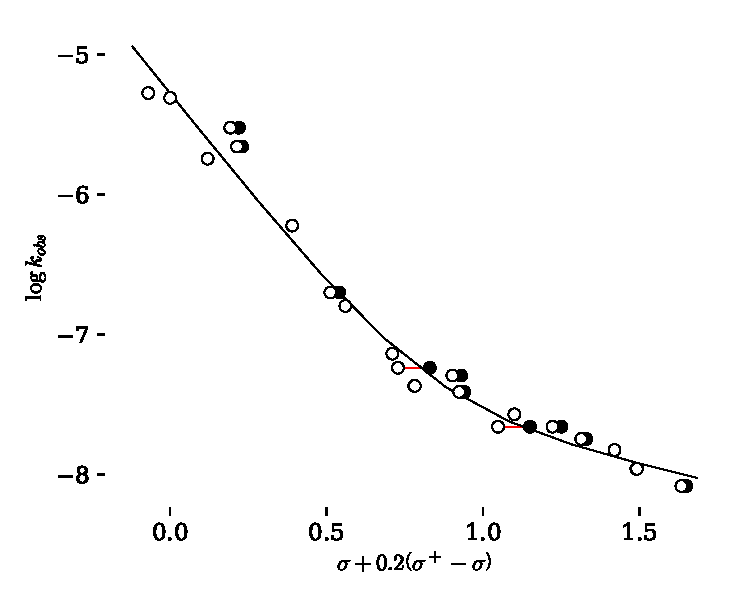
\includegraphics[scale=0.8]{images/plot11.pdf}
  \caption[-5mm]{Yukawa-Tsuno plot for the $\rm S_N2$ set of rates.  \vspace{2mm} \\
  {$r = 0.21$}: white circles  \\
  \hspace{3mm} $\rho_1 = -2.8 \pm 0.27$,   \\
  \hspace{3mm} $\rho_2 = -0.52 \pm 0.32$, $R^2 = 0.983$ \vspace{2mm} \\
  {$r = 0$}: black circles  \\
  \hspace{3mm} Shown for comparison. \vspace{2mm} \\

   
 } 
  \label{fig:YK5}
\end{figure}

\begin{marginfigure}[-25mm]
  \centering
    \caption[-0mm]{Optimizing $r$ for the Yukawa-Tsuno plot \label{fig:YK5R}}  
    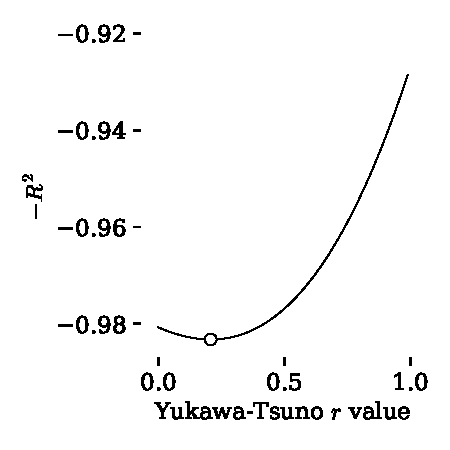
\includegraphics[width=150pt]{images/plot11R.pdf}
\end{marginfigure}



\subsection{The Holistic Yukawa-Tsuno Plot}

We will now unite the two data sets and fit the results to a model that includes both reactions. The data set will use the calculated values for $\sum \sigma$ based on the Yukawa-Tsuno term for $\sigma$. The $\sigma_m$ values do not have a resonance connection to the reaction centre but the $\sigma_p$ values in each reactant will be calculated using the $r$ values of 1.4 or 0.2 according to the putative mechanism.

\clearpage
The model is shown in eq.~\ref{eq:YKmodel}. It is just the same model as eq.~\ref{eq:1} with a third reaction term added. 

\begin{equation}
\begin{split}
\log{k_{{S_N2}_A}} &= \rho_{{S_N2}_A} \sum \sigma_{S_N2} + c_{{S_N2}_A} \\
\log{k_{{S_N2}_B}} &= \rho_{{S_N2}_B} \sum \sigma_{S_N2} + c_{{S_N2}_B} \\
\log{k_{S_N1}} &= \rho_{S_N1} \sum \sigma_{S_N1} + c_{S_N1} \\
\sigma_{S_N2} &= \sigma + 0.2(\sigma^+ - \sigma) \\
\sigma_{S_N1} &= \sigma + 1.4(\sigma^+ - \sigma) \\
\log{k_{obs}} &= \log\left(10^{k_{S_N1}} + 10^{k_{{S_N2}_A}} + 10^{k_{{S_N2}_B}}\right)
\label{eq:YKmodel}
\end{split}
\end{equation}

The plot of the combined sets of data for both reaction mechanism paired with the corresponding calculated $\sigma$ values is shown in figure~\vref{fig:YK6}.

\begin{figure}[h!]
  \centering
  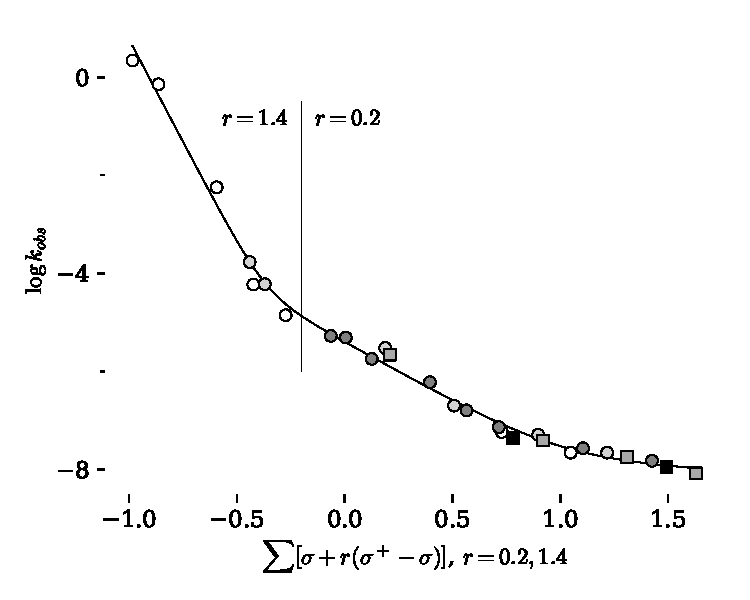
\includegraphics[scale=0.8]{images/plot12.pdf}
  \caption[-5mm]{Yukawa-Tsuno plot for the $\rm S_N2$ set of rates using $r$ values determined in figures~\ref{fig:YK4} and \ref{fig:YK5}.  \vspace{2mm} \\
  \ce{p-MeO}: white circles  \\
  \ce{p-Me}: light gray circles  \\
  \ce{p-H}: dark gray circles  \\
  \ce{p-Br}: gray squares   \\
  \ce{p-NO2}: black squares  \vspace{2mm}  \\

 {$r_{S_N1} = 1.4$} and {$r_{S_N2} = 0.2$} \vspace{2mm}  \\
 $\rho_{{S_N1}} = -8.35 \pm 0.46$,   \\
 $\rho_{{S_N2}_A} = -2.44 \pm 0.29$,   \\
 $\rho_{{S_N2}_B} = -0.29 \pm 0.62$, $R^2 = 0.994$ \vspace{2mm} \\
 } 
\label{fig:YK6}
\end{figure}

We can clearly see both mechanistic regimes here. The $\rm S_N1$ mechanism is occurring the the region where the calculated $\sum \sigma$ value is less than $-0.25$ and we observe a slope of $\rho_{{S_N1}} = -8.35 \pm 0.46$. This is the same magnitude of negative slope that the authors observed in the data that they deemed to be due to the the $\rm S_N1$ mechanism. The $\rm S_N2$ mechanism is observed when $\sum \sigma > -0.25$. The slope, $\rho_{S_N2}$, in this region is much lower in magnitude. A slope of $\rho_{S_N2} = -2.44 \pm 0.29$ is observed in the most activated reactants and indicate a TS with a slight positive charge developing on the benzyl carbon. The slope of $\rho_{S_N2} = -0.29 \pm 0.62$ observed in the least activated reactants indicates a tighter $\rm S_N2$ TS with essentially no charge buildup at the reaction centre. The change in slope indicates that the structure of the transition state changes as electron density in the ring changes. The more electron dense systems are able to stabilize some positive charge at the benzylic carbon and the TS is loose compared to the less electron dense cases. See figure~vref{fig:mech1} for a reaction scheme that illustrates this concept.

\subsection{Product Analysis Yukawa-Tsuno-Style}

The authors plotted the reaction selectivity with solvent nucleophiles for each \textit{para} substituted series separately and used the slope of the plot to identify the reactants that likely reacted via $\rm S_N1$ mechanism. They identified that the \ce{p-OMe} series was capable of stabilizing the $\rm S_N1$ carbocation intermediate. In my own analysis I hypothesized that the more electron-rich versions of the \ce{p-Me} series also reacted predominantly via  $\rm S_N1$. I used this set of $\rm S_N1$ to determine the Yukawa-Tsuno $r$ value based on when the proposed $\rm S_N1$ data lined up. This is not the most robust approach, but the result is backed up by how well the $r$ value places the $\rm S_N1$ data with respect to the $\rm S_N2$ data. 

Can we interpret the product analysis results using the Yukawa-Tsuno calculated values for $\sum \sigma$ with $r = 0.2$ for the $\rm S_N2$ data and $r = 1.4$ for the $\rm S_N1$ data set. Figure~\vref{fig:YK7} shows this plot. 

\begin{figure}[h!]
  \centering
  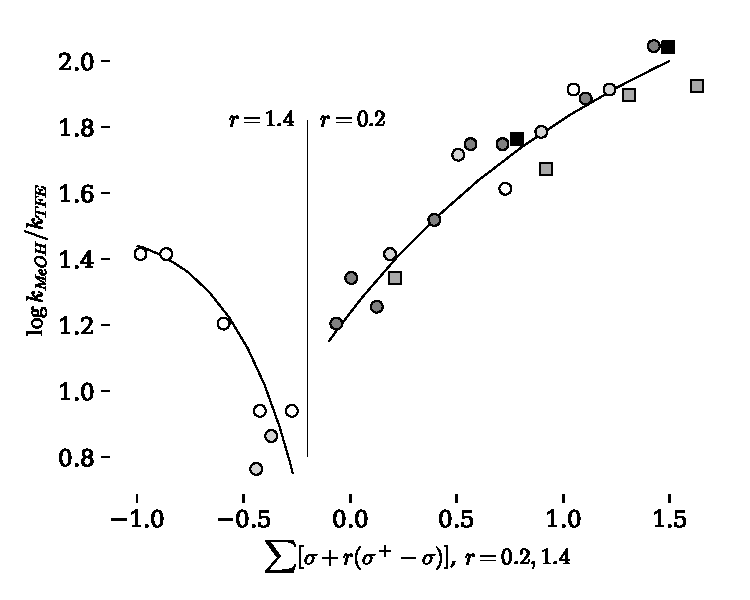
\includegraphics[scale=0.8]{images/plot13.pdf}
  \caption[-5mm]{Product analysis plotted with the same Yukawa-Tsuno $x$-axis as used in figure~\ref{fig:YK6}. Compare this presentation with the same data plotted according to the authors' method in figure~\ref{fig:fig3-4_paper}.  \vspace{2mm} \\
  \ce{p-MeO}: white circles  \\
  \ce{p-Me}: light gray circles  \\
  \ce{p-H}: dark gray circles  \\
  \ce{p-Br}: gray squares   \\
  \ce{p-NO2}: black squares   \vspace{2mm}  \\

 The line is hand drawn and has no meaning beyond my attempt to prejudice your eyes and force you to believe my interpretation of the data. I wasn't able to come up with a mathematical model beyond a crude interpolation. 
 } 
\label{fig:YK7}
\end{figure}

We see that the series of reactants line up nicely in a pattern that parallels the results plotted in figure~\ref{fig:YK6}. We observe a negative slope as the carbocation intermediate of the $\rm S_N1$ mechanism becomes more reactive and less selective with decreasing electron density. Then the slope switches to positive when we enter the $\rm S_N2$ regime as the reaction becomes slower and more selective.\sidenote[][-30mm]{There is a nice discussion of this idea on page 452 of the textbook where one of those interesting ``connections'' highlights is presented featuring solvolysis of 1-phenyl-1-chloro-ethane (benzyl chloride with a single methyl group attached to the benzylic carbon. This is work by the very author of the paper that this exploration is based upon, but from 40 years ago. It seems he is back to his old stomping grounds. Note that this previous work was done in the laboratory of Bill Jencks, one of the absolute giants of physical organic chemistry. Cool!} The two proposed $\rm S_N1$ cases from the \ce{p-Me} series fit nicely in with the \ce{p-OMe} series. they are actually even less selective and one could say that the \ce{p-Me} substituent does not stabilize the carbocationic intermediate as well as the \ce{p-OMe} substituent as so this is consistent with our expectations.

\section{Comments and Conclusions}

Let us now consider how well we reproduced the authors' analysis and how our own re-analysis of the data provided insight into the reaction mechanism. First, here is a quick overview of the authors results and conclusions.

\subsection{Summary of the Paper}

The authors subdivided their data into five series of \textit{para} substituted benzyl chlorides. They essentially constructed a two dimensional grid with one axis being substituent parameters for the \textit{meta} substituents on each ring ($\sum \sigma_m$) and the other being the substituent constant for the resonance effect of the \textit{meta} ($\sigma_r$). 

Along the axis \textit{meta} substituents they determined a set of reaction constants that revealed the substituent effect in each series. The $\rho_n$ value had a very large magnitude for the \ce{p-OMe} series, which indicated that this series reacted predominantly via the $\rm S_N1$ mechanism. The product analysis revealed how the selectivity for solvent nucleophiles changed with substituents, and the authors concluded that the two least activated reactants in the \ce{p-OMe} series were cases of the $\rm S_N2$ mechanism. All the other series were concluded to be $\rm S_N2$ with a progressive change in TS structure as electron density decreased.\marginnote[0mm]{{\sc{\textbf{Personal Exploration Tip:}}} Provide a closing argument where you summarize your key points and brag about how smart you are while twisting the knife with some final jabs at the authors' hard work. But thats my style; you might choose to be more positive.}

The authors then plotted the data along the $\sigma_r$ axis and showed that the reactants that possessed more activating \textit{meta} substituents has a much greater dependance of resonance effects of the \textit{para} substituent as expressed by the $\sigma_r$ value.  

The two-parameter system that they used was the extended Hammett equation. It will yield a value for sensitivity to polar (inductive) effects, $\rho_n$ and to resonance effects, $\rho_r$. The authors used a set of substituent constants, $\sigma^n$, that represent the polar effect of a substituent in the para position to enable them to calculate a value for the resonance contribution by subtracting these $\sigma^n$ from the $\sigma^+$ value which includes both inductive and resonance effects. They showed that the system had a steeply increasing requirement for resonance stabilization as the electron density on the ring increased. 

Because the mechanism is changing across the data set (and the TS structure in the $\rm S_N2$ regime is changing too), the authors ended up with a set of five values for each of $\rho_n$ and $\rho_r$. these values were discussed and do back up the conclusion that the solvolysis of benzyl chloride proceeds through an $\rm S_N2$ mechanism but that a $\rm S_N2$ predominates in the more activated reactants.

\subsection{Criticism}

The authors approach was sound but they provided little information for the details of the data analysis. I presume that the curves presented by the authors are mostly apocryphal as they only report slopes for linear fits of selected regions of each data series. My own versions of their plots for $\rho_n$ produced values that were very close to those in the paper (although one needed to delete a datapoint to get exactly the same values.) The plots for $\rho_r$ produced very different values for the most deactivating series of \textit{meta} substituents. I was unable to reproduce these results using the authors own data. Perhaps I misunderstood their methodology or perhaps the figure in the paper is in error? Without documented data analysis (preferably the code and data that will reproduce the plot anywhere) I cannot say much more. My values do not contradict the authors' conclusions, they are just different with no clear reason why.

The authors report no precision for the parameters obtained from their line fits. My own reproduction of their methods reveal quite large standard errors for all parameters (approaching $\pm$\qty{10}{\percent} of the values in the $\rho_n$ values and $\pm$\qty{50}{\percent} in the $\rho_r$ values.) When one splits the data set up into many smaller sets, the small numbers of data points will inevitably lead to larger standard errors in line fits.

In the end, it all comes down to the lack of documentation of the data analysis methods. As chemists, we obsess about experimental procedure, but the data analysis procedure are just as important. I hope that you will see that using a \textit{Python} notebook will allow the reader to run the code and get exactly the same plots and results. If an error is found, the code can be adjusted and the correct plot quickly demonstrated. 

\subsection{Summary of this Exploration}

I wondered if all of this data could be presented more simply and draw the same conclusions. I chose to use the Yukawa-Tsuno plot, which is also a two-parameter plot but expressed the separate dependance of resonance by the $r$ value. The YK plot really just allows us to explore the continuum between systems that do not require resonance stabilization at the reaction centre (where $\sigma$ values are used) and systems that require such stabilization (where $\sigma^+$ or $\sigma^-$ values are used.) \marginnote[-100mm]{{\sc{\textbf{Personal Exploration Tip:}}} After writing your exploration and praising the work or venting your frustrations, you should read it. Does it flow well? Does the narrative tell a story with a beginning, middle and (most importantly) an end? Is it more than ten pages of text? Then, it is time to edit. Trim your story and carve away anything unnecessary. You may have to cut a whole line of thought that you spent hours on. 

This exploration is much too long. What should I leave on the cutting-room floor? I think I might delete my discussion of the product analysis (the ratios of product in the 7-/27/3 solvent mixture.) I could also drop the plot and discussion of the Brown-Okamoto plot since I was on my way to Yukawa-Tsuno anyway. How would you trim this exploration down. 

Remember, the Schneider cut was a bloated exercise in vanity. All movies should be 90 minutes. In the early days of the movies, the director was fired right after the last reel of film was in the can and the editor made the movie. Always write freely and too much, then edit it down.}

I still had to bin the data into two series, the $\rm S_N1$ series and the $\rm S_N2$. I proposed that the two most activated reactants in the \ce{p-Me} series were $\rm S_N1$ and this hypothesis allowed me to fit the $\rm S_N1$ data to determine the $r$ value. I would not have been able to do that otherwise. We need at least two different \textit{para} substituents that have values for $\sigma^+$ parameters if we are to fit for $r$. The $r$ value was larger than 1.0, indicating a carbocation intermediate of high energy, like a primary benzyl cation.

Then I optimized the $r$ value in the $\rm S_N2$ series. The value was small and the plot quality was hardly diminished if it was set to zero. This is expected for the $\rm S_N2$ mechanism, where there is no empty orbital in the TS to receive electron density via resonance.

All of the data was plotted together using $\sigma$ values calculated according to the YK equation with $r = 1.4$ for the $\rm S_N1$ cases and $r = 0.2$ for the $\rm S_N2$ cases. The expected slopes for a $\rm S_N1$ and $\rm S_N2$ mechanism were observed and the slope in the $\rm S_N2$ section changed as the TS moved from a looser to a tighter configuration with lower electron density.

The nucleophilic selectivity was plotted against the same $x$-axis and revealed the same information as the YK plot. Rather than plotting ten different series and getting five pairs of $\rho$ values from the extended Hammett equation, followed up by four separate plots for the nucleophile selectivity, I plotted two plots, both having the same $x$-axis. I could easily have plotted both the YK plot and the selectivity plot in the same figure. 

It could have saved a lot of pages if the authors of this paper had used my own method. I would also have put the four pages of synthesis methodology in the supplementary material along with the \textit{Python} notebooks that document all my data analysis. I believe I could have trimmed that paper from fifteen pages to just six.\sidenote[][0mm]{Who am I to count pages? This exploration just hit 20 pages and I'm not done yet.}

\subsection{Comments}

The Yukawa-Tsuno analysis provides the same conclusions and, in my humble opinion, is more easily understood. It also revealed the likelihood that the \ce{p-Me} series could proceed by the $\rm S_N1$ when meta substituents are also electron-donating. I feel that the YK approach was superior. 

I had promised to interpret the results using other LFER systems such as the Swain-Lupton multi-parameter plot.\marginnote[-10mm]{The Swain-Lupton equation $$\log{\frac{k_X}{k_H}} = fF + rR$$ where $F$ and $R$ are substituent parameters that describe inductive field effects and resonance effects. $f$ and $r$ are reaction constants that establish the relative sensitivity of the system to each set of substituent parameters. 

Compare this to the extended Hammett equation used by Yeary and Richard which was presented way back on the first page of this overlong exploration. Its been so long since we were there that I will reproduce that equation below...

$$
\log{\frac{k_X}{k_H}} = \rho_n \sigma_n + \rho_r \sigma_r
$$ \vspace{2mm}
} However this exploration can't go on forever, so I will leave that as an exercise for the reader.

\subsection{One Final Rant}

Finally, the authors used designations for the mechanisms that I found unfamiliar. We are used to these solvolysis reactions being described as $\rm S_N1$ or $\rm S_N2$. The authors used the terms $\rm D_N + A_N$  and $\rm D_NA_N$ to describe the mechanisms. I looked into this and found a review by the great Bill Jencks himself along with another giant of physical organic chemistry, Robert Guthrie, in which they propose new nomenclature for reaction mechanisms.\sidenote[][0mm]{``IUPAC recommendations for the representation of reaction mechanisms.''
R.D. Guthrie, W.P. Jencks.
\textit{Acc. Chem. Res.}, \textbf{1989}, \textit{22}, 343-349.
\url{https://doi.org/10.1021/ar00166a001}} They urged chemists to abandon the less precise nomenclature established by Kieth Ingold twenty years previously. Their effort was clearly unsuccessful and we still use Ingold's $\rm S_N1$ and $\rm S_N2$ to describe these reactions. John Richard is disciple of Jencks and is clearly carrying the torch here for this nomenclature system. Perhaps persistence will overcome momentum? I don't think any of us will live to see that day.


\nobibliography{}

\end{document}